\chapter{Mô tả hệ thống}

\section{Kiến trúc tổng quát của hệ thống}
Để giải quyết các vấn đề đã được trình bày ở mục \ref{sec:muctieu},
hệ thống ứng dụng Chatbot tư vấn có các thành phần chính đó là phần
giao diện giao tiếp với người dùng, dữ liệu thời trang phục vụ cho
việc tư vấn và phần lõi của hệ thống. Mối quan hệ giữa các thành phần
được biểu diễn như hình \ref{fig:chatbotapp}

\begin{figure}[ht!]
    \centering
    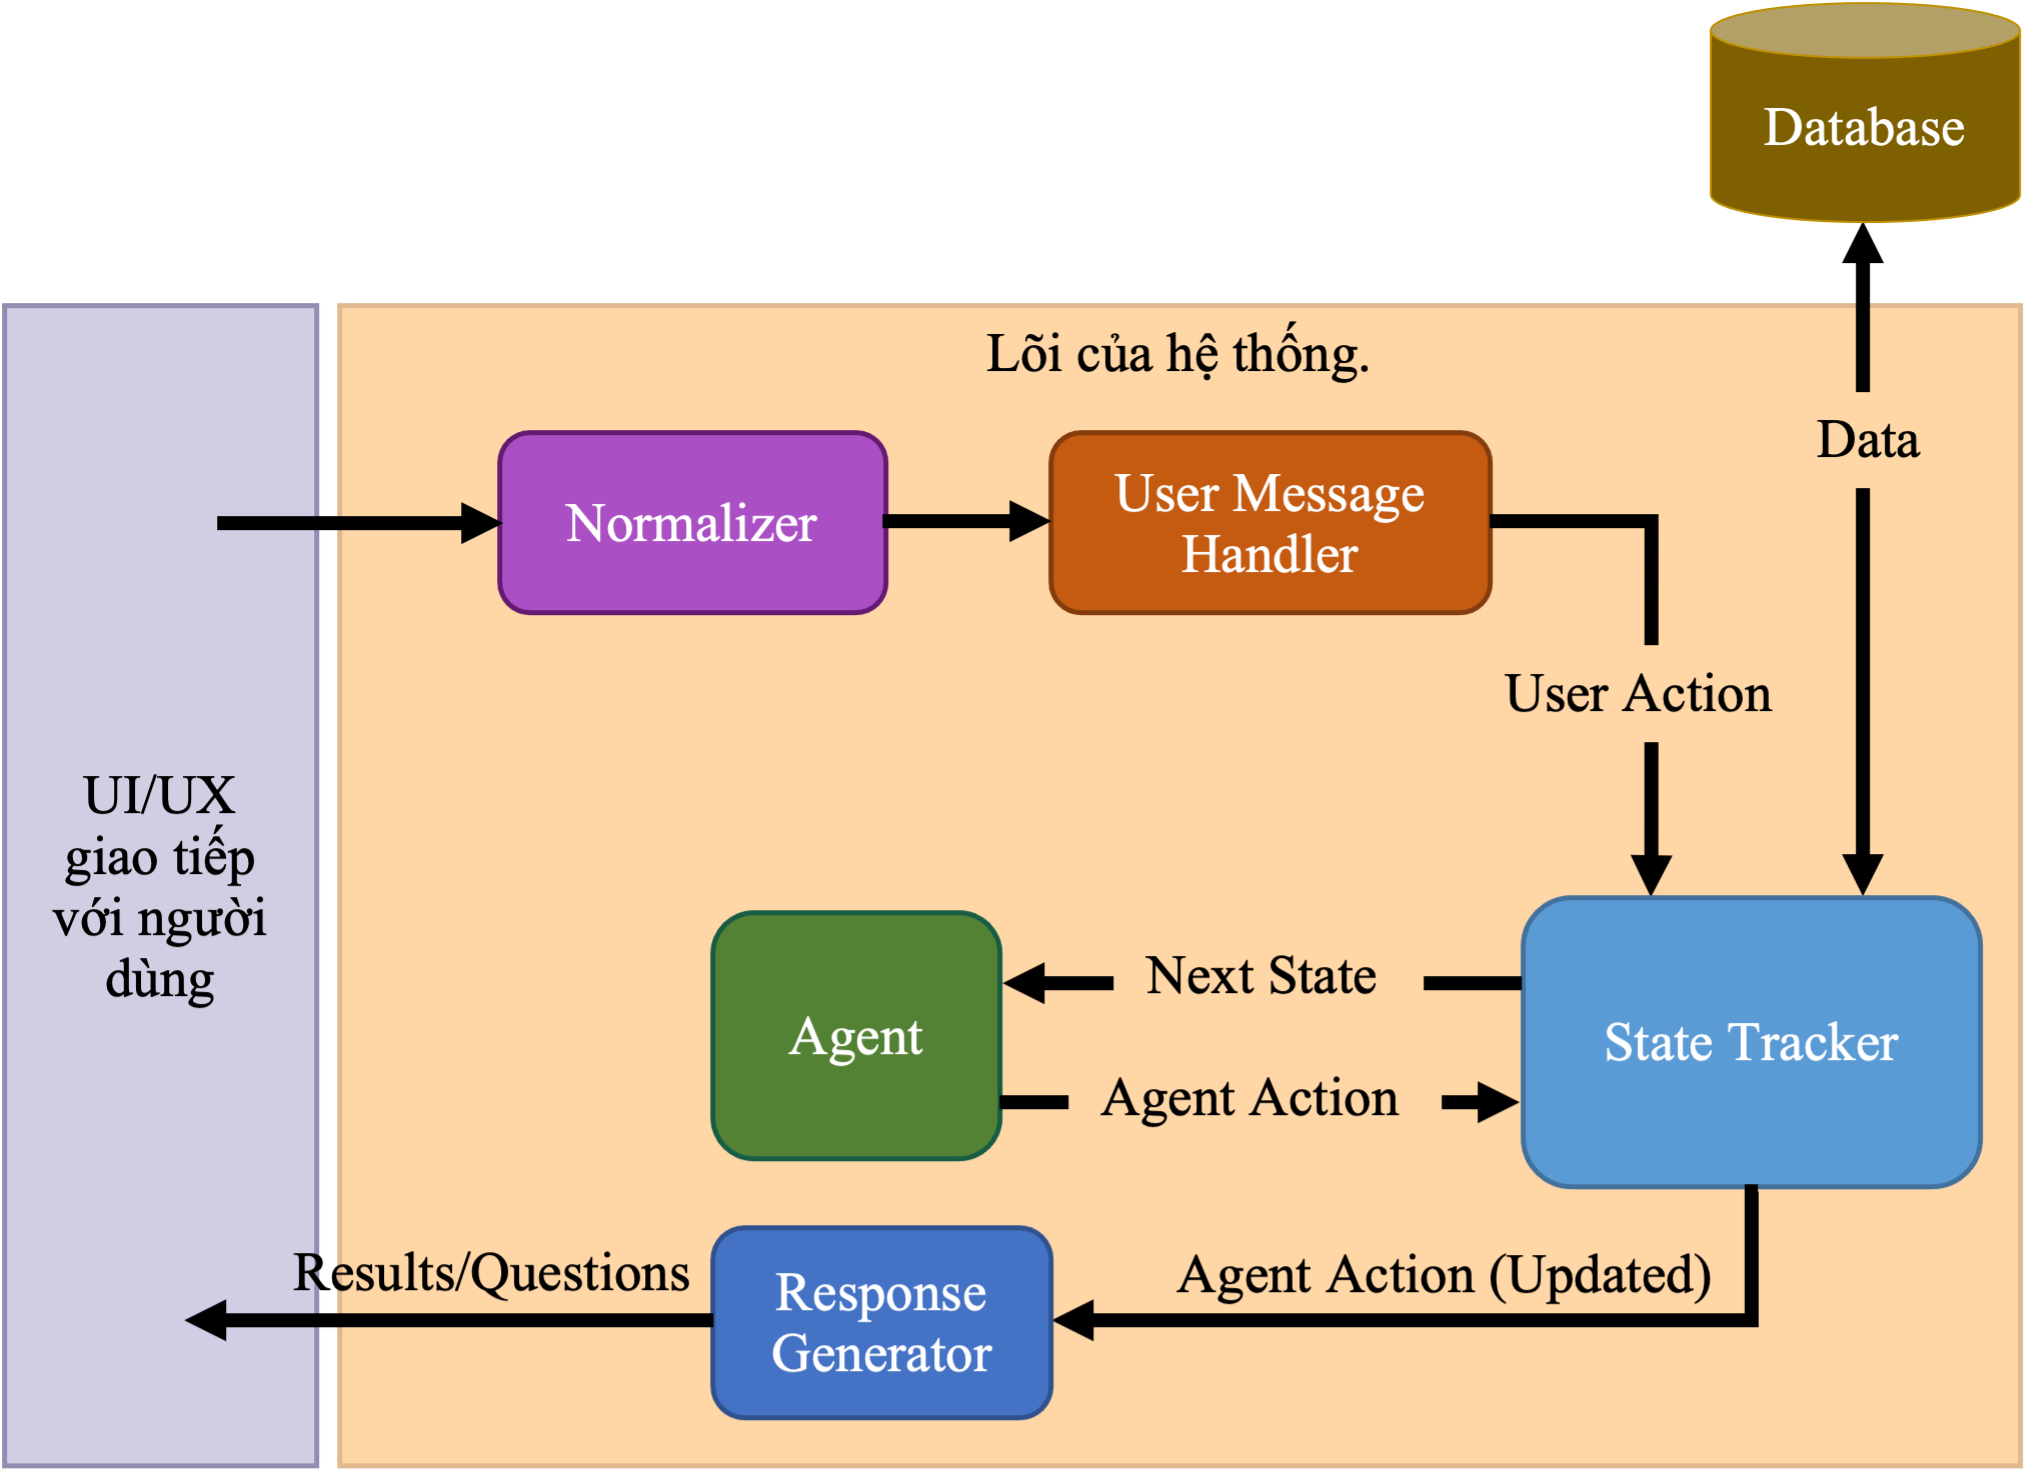
\includegraphics[scale=0.95]{thesis/chatbot/phuongphap/img/chatbot_app.png}
    \caption{Kiến trúc tổng quát của hệ thống Chatbot}
    \label{fig:chatbotapp}
\end{figure}

Trong phần lõi của hệ thống, ta có các phần con khác được mô tả
cụ thể sau đây:

\begin{itemize}
    \item \textbf{Normalizer (Bộ chuẩn hóa dữ liệu):} dữ liệu
    sau khi nhận được từ người dùng sẽ được chuẩn hóa để thống nhất
    về cách biểu diễn trước khi tạo \textit{User Action} (hành động
    của người dùng) và lưu vào cơ sở dữ liệu.
    \item \textbf{User Message Handler (Bộ xử lý phản hồi
    người dùng):} có nhiệm vụ tạo ra \textit{User Action}.
    \item \textbf{State Tracker (Bộ quản lý trạng thái hội thoại):}
    có nhiệm vụ giám sát trạng thái hiện tại của cuộc hội thoại để
    cung cấp thông tin cho \textit{agent} (tác nhân) ra quyết định,
    đồng thời thực hiện truy xuất vào cơ sở dữ liệu để lấy các
    thông tin cần thiết trước khi gửi kèm nó cùng với phản hồi
    từ \textit{agent}.
    \item \textbf{Agent (Bộ sinh phản hồi):} có nhiệm vụ dựa vào
    trạng thái hiện tại mà \textit{State Tracker} cung cấp để đưa ra
    quyết định phản hồi một hành động cụ thể và gửi về lại
    \textit{State Tracker}.
    \item \textbf{Response Generator (Bộ sinh câu phản hồi):} có
    nhiệm vụ chuyển đổi \textit{Agent Action} nhận từ
    \textit{State Tracker} tạo ra câu phản hồi dưới dạng ngôn ngữ
    tự nhiên trước khi gửi về cho người dùng.
\end{itemize}

\section{Sơ đồ tình huống sử dụng (Use Case Diagram)}

\begin{figure}[ht!]
    \centering
    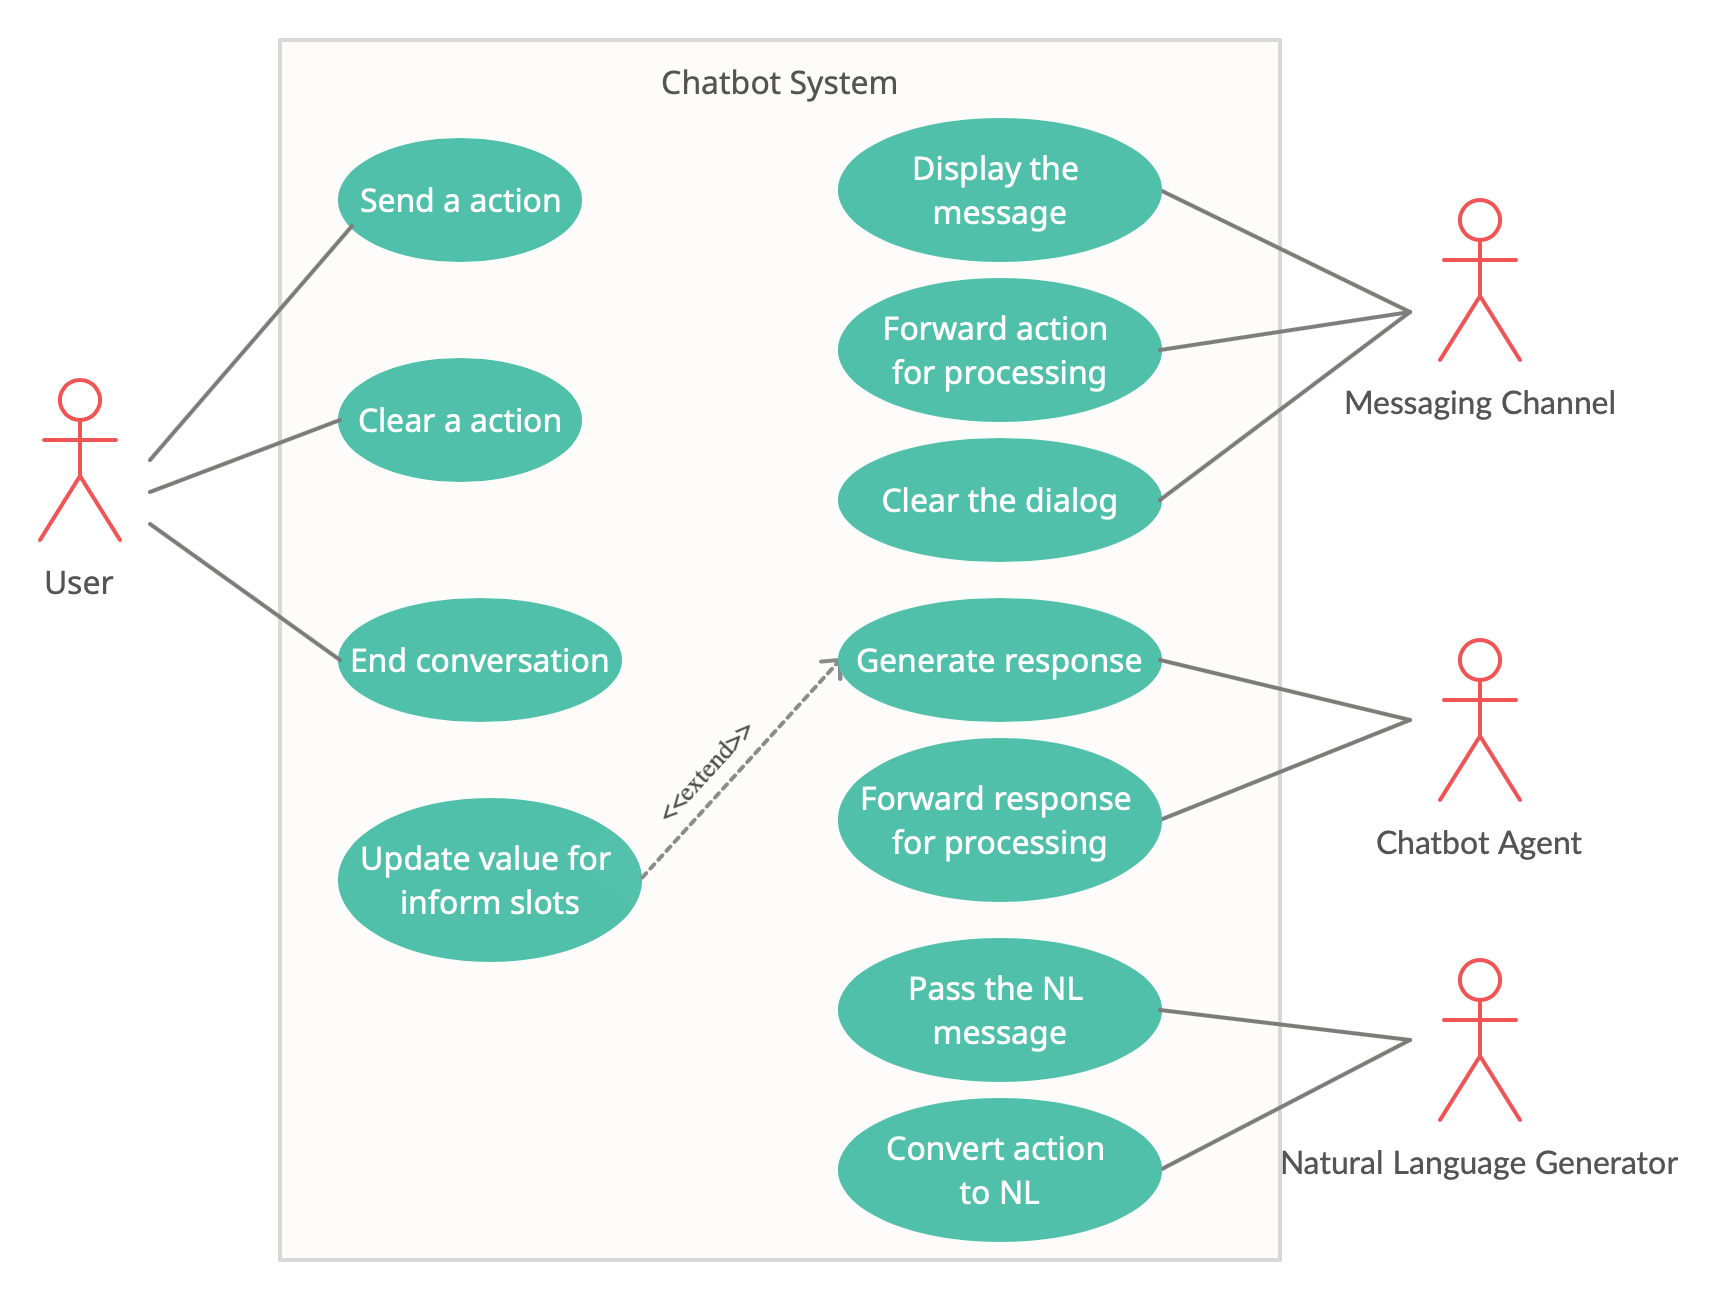
\includegraphics[scale=0.25]{thesis/chatbot/phuongphap/img/use_case.png}
    \caption{Sơ đồ tình huống sử dụng (Use Case Diagram) của hệ thống
    Chatbot}
    \label{fig:usecase}
\end{figure}

Sơ đồ tình huống sử dụng (Use Case Diagram) của hệ thống Chatbot được
diễn tả ở hình \ref{fig:usecase}. Có các thành phần cụ thể như sau:

\begin{itemize}
    \item \textbf{Actor:}
    \begin{itemize}
        \item \textbf{User:} Người dùng cuối của Chatbot. Giao tiếp
        với hệ thống thông qua giao diện Chatbot.
        \item \textbf{Messaging Channel:} Kênh thông tin liên lạc
        giữa người dùng và tác nhân.
        \item \textbf{Chatbot Agent:} Tác nhân sinh ra câu phản hồi
        cho người dùng.
        \item \textbf{Natural Language Generator:} Bộ tạo ra các câu
        phản hồi dưới dạng ngôn ngữ tự nhiên.
    \end{itemize}
    \item \textbf{Use case:}
    \begin{itemize}
        \item \textbf{Send a action:} Đối tượng thực hiện (actor) là
        \textit{User}. Đây là hành vi gửi đi một hành động có thể là
        yêu cầu, thông báo, xác nhận thông tin về sản phẩm của
        người dùng.
        \item \textbf{Clear a action:} Đối tượng thực hiện là
        \textit{User}. Xóa đi một hành động tạm thời đang thực hiện
        nhưng chưa được gửi đi.
        \item \textbf{End conversation:} Đối tượng thực hiện là
        \textit{User}. Yêu cầu kết thúc cuộc hội thoại hiện tại.
        \item \textbf{Forward action for processing:} Đối tượng
        thực hiện là \textit{Messaging Channel}. Đây là hành vi
        chuyển tiếp một hành động của người dùng sang bộ sinh
        ngôn ngữ tự nhiên.
        \item \textbf{Display the message:} Đối tượng thực hiện là
        \textit{Messaging Channel}. Hiển thị các câu thoại trên
        giao diện hội thoại.
        \item \textbf{Clear the dialog:} Đối tượng thực hiện là
        \textit{Messaging Channel}. Xóa toàn bộ lịch sử và nội dung
        cuộc hội thoại trên giao diện hội thoại.
        \item \textbf{Generate response:} Đối tượng thực hiện là
        \textit{Chatbot Agent}. \textit{Agent} dựa vào trạng thái
        hiện tại của hội thoại quyết định một hành động phản hồi.
        \item \textbf{Update value for inform slots:} Đối tượng
        thực hiện là \textit{Chatbot Agent}. Tùy vào hành động
        hiện tại của \textit{agent}, nếu có thông tin cần thông báo
        cho người dùng, nó sẽ truy vấn vào cơ sở dữ liệu tìm ra
        giá trị phù hợp cho thông tin đó.
        \item \textbf{Forward response for processing:} Đối tượng
        thực hiện là \textit{Chatbot Agent}. Đây là hành vi
        chuyển tiếp một hành động của \textit{agent} sang bộ sinh
        ngôn ngữ tự nhiên.
        \item \textbf{Convert action to NL:} Đối tượng thực hiện là
        \textit{Natural Language Generator}. Chuyển đổi hành động
        của người dùng và \textit{agent} sang ngôn ngữ tự nhiên.
        \item \textbf{Pass the NL message:} Đối tượng thực hiện là
        \textit{Natural Language Generator}. Hành động chuyển
        câu thoại sang kênh hội thoại.
    \end{itemize}
\end{itemize}

\section{Các ý định của người dùng}
Ý định người dùng là khái niệm nói về nhu cầu của người dùng thể hiện
qua câu thoại. Ý định người dùng có thể đơn giản chỉ là chào hỏi,
cảm thán hoặc yêu cầu về một thông tin thành phần nào đó của sản phẩm
như chất liệu, màu sắc, ... Trong mục này, mô tả các ý định người dùng
được định nghĩa trong đề tài.

\subsection{Chào hỏi}
\begin{itemize}
    \item \textbf{Mô tả:} Đây là ý định khi người dùng thực hiện các
    câu chào, hỏi thăm với cửa hàng (tác nhân Chatbot).
    \item \textbf{Ví dụ:}
    \begin{itemize}
        \item Hi shop nhé
        \item Chào bạn
    \end{itemize}
    \item \textbf{Phản hồi:} Tác nhân sẽ thực hiện câu chào phản hồi
    lại khách hàng.
\end{itemize}

\subsection{Kết thúc}
\begin{itemize}
    \item \textbf{Mô tả:} Đây là ý định khi người dùng muốn kết thúc
    cuộc hội thoại, thường là một câu chào tạm biệt.
    \item \textbf{Ví dụ:}
    \begin{itemize}
        \item Ok bye shop
        \item Bye shop nhé
    \end{itemize}
    \item \textbf{Phản hồi:} Tác nhân sẽ thực hiện câu tạm biệt
    phản hồi lại khách hàng.
\end{itemize}

\subsection{Cảm ơn/ Đồng tình}
\begin{itemize}
    \item \textbf{Mô tả:} Đây là ý định khi người dùng thể hiện ý
    đồng tình, hoặc cảm ơn câu phản hồi của tác nhân.
    \item \textbf{Ví dụ:}
    \begin{itemize}
        \item Ok shop
        \item Cảm ơn bạn
    \end{itemize}
    \item \textbf{Phản hồi:} Sau khi nhận được ý định này từ
    khách hàng, tác nhân cập nhật thông tin vào hệ thống và tiếp tục
    tiến trình cuộc hội thoại.
\end{itemize}

\subsection{Phản đối}
\begin{itemize}
    \item \textbf{Mô tả:} Đây là ý định khi người dùng thể hiện ý
    không đồng tình, phản đối câu phản hồi của tác nhân.
    \item \textbf{Ví dụ:}
    \begin{itemize}
        \item Không phải shop ạ
        \item Mình không cần
    \end{itemize}
    \item \textbf{Phản hồi:} Sau khi nhận được ý định này từ
    khách hàng, tác nhân cập nhật thông tin vào hệ thống và
    tiếp tục tiến trình cuộc hội thoại.
\end{itemize}

\subsection{Yêu cầu thông tin màu sắc}
\begin{itemize}
    \item \textbf{Mô tả:} Mỗi mẫu sản phẩm có nhiều màu khác nhau,
    phù hợp cho nhiều sở thích của khách hàng. Đây là ý định
    phát sinh khi khách hàng đặt câu hỏi với mục đích muốn có
    thông tin về các màu của sản phẩm.
    \item \textbf{Ví dụ:}
    \begin{itemize}
        \item Áo hoa này có những màu gì vậy ạ?
        \item Cho mình xin các màu của sản phẩm này
    \end{itemize}
    \item \textbf{Phản hồi:} Sau khi thu thập đủ các thông tin,
    phản hồi trả về cho khách hàng sẽ là thông tin màu sắc của
    sản phẩm có thể có, những sản phẩm này phải thỏa các điều kiện
    ràng buộc tìm được trong cơ sở dữ liệu.
\end{itemize}

\subsection{Yêu cầu thông tin chất liệu}
\begin{itemize}
    \item \textbf{Mô tả:} Mỗi mẫu sản phẩm có thể được làm bởi mỗi
    loại vật liệu khác nhau, phù hợp cho nhu cầu của khách hàng.
    Đây là ý định phát sinh khi khách hàng đặt câu hỏi với mục đích
    muốn có thông tin về chất liệu của sản phẩm.
    \item \textbf{Ví dụ:}
    \begin{itemize}
        \item Chất vải là gì vậy ạ?
        \item Đầm này vải gì vậy shop?
    \end{itemize}
    \item \textbf{Phản hồi:} Sau khi thu thập đủ các thông tin,
    phản hồi trả về cho khách hàng sẽ là thông tin chất liệu của
    sản phẩm, những sản phẩm này phải thỏa các điều kiện ràng buộc
    tìm được trong cơ sở dữ liệu.
\end{itemize}

\subsection{Yêu cầu thông tin giá bán}
\begin{itemize}
    \item \textbf{Mô tả:} Mỗi mẫu sản phẩm có thể được bán với các
    giá khác nhau, tùy vào chất liệu, màu sắc và các chi phí
    phát sinh khác. Đây là ý định phát sinh khi khách hàng đặt
    câu hỏi với mục đích muốn có thông tin về giá bán của sản phẩm.
    \item \textbf{Ví dụ:}
    \begin{itemize}
        \item Nguyên bộ này hết nhiêu tiền?
        \item Áo thun này bao tiền vậy
    \end{itemize}
    \item \textbf{Phản hồi:} Sau khi thu thập đủ các thông tin,
    phản hồi trả về cho khách hàng sẽ là thông tin giá bán có thể có
    của sản phẩm, những sản phẩm này phải thỏa các điều kiện
    ràng buộc tìm được trong cơ sở dữ liệu.
\end{itemize}

\subsection{Yêu cầu thông tin tình trạng sản phẩm}
\begin{itemize}
    \item \textbf{Mô tả:} Tại mỗi thời điểm, cửa hàng có thể có những
    mẫu sản phẩm khác nhau. Việc một số sản phẩm có thể không còn
    hoặc tạm hết trong kho của cửa hàng. Đây là ý định phát sinh khi
    khách hàng đặt câu hỏi với mục đích muốn xác nhận rằng sản phẩm
    vẫn còn được bán bởi cửa hàng.
    \item \textbf{Ví dụ:}
    \begin{itemize}
        \item Đầm caro còn không shop
        \item Áo này còn màu xanh không?
    \end{itemize}
    \item \textbf{Phản hồi:} Sau khi thu thập đủ các thông tin,
    phản hồi trả về cho khách hàng sẽ là thông tin hiện tại của
    sản phẩm, những sản phẩm này phải thỏa các điều kiện ràng buộc
    tìm được trong cơ sở dữ liệu.
\end{itemize}

\subsection{Thông báo về tên sản phẩm}
\begin{itemize}
    \item \textbf{Mô tả:} Tên sản phẩm là thông tin quan trọng nhất
    trong hoạt động tư vấn. Khi bắt đầu cuộc hội thoại tư vấn,
    khách hàng sẽ có mục tiêu tư vấn cho một sản phẩm nhất định.
    Đây là ý định phát sinh khi khách hàng thông báo cho shop về
    sản phẩm mình muốn tìm hiểu.
    \item \textbf{Ví dụ:}
    \begin{itemize}
        \item Bộ set vest cổ xéo shop ơi.
        \item Mình muốn tư vấn đầm hoa này ạ
    \end{itemize}
    \item \textbf{Phản hồi:} Sau khi nhận được ý định này từ
    khách hàng, tác nhân cập nhật thông tin vào hệ thống và
    tiếp tục tiến trình cuộc hội thoại.
\end{itemize}

\subsection{Thông báo về màu sắc}
\begin{itemize}
    \item \textbf{Mô tả:} Sau khi có được các thông tin về sản phẩm
    mong muốn của khách hàng. Họ có thể sẽ muốn đặt mua một sản phẩm
    có màu cụ thể như yêu cầu. Đây là ý định phát sinh khi khách hàng
    muốn đặt mua sản phẩm và thông báo cho shop về màu sắc của
    sản phẩm cần lấy.
    \item \textbf{Ví dụ:}
    \begin{itemize}
        \item Mình lấy cái màu đen này nha.
        \item Cái set vest này mình lấy màu trắng.
    \end{itemize}
    \item \textbf{Phản hồi:} Sau khi thu thập đủ các thông tin,
    phản hồi trả về cho khách hàng sẽ là toàn bộ thông tin về
    sản phẩm mà khách hàng đã đặt, những sản phẩm này phải thỏa
    các điều kiện ràng buộc tìm được trong cơ sở dữ liệu.
\end{itemize}

\subsection{Thông báo về kích cỡ}
\begin{itemize}
    \item \textbf{Mô tả:} Sau khi có được các thông tin về sản phẩm
    mong muốn của khách hàng. Họ có thể sẽ muốn đặt mua một sản phẩm
    có kích cỡ cụ thể như yêu cầu. Đây là ý định phát sinh khi
    khách hàng muốn đặt mua sản phẩm và thông báo cho shop về
    kích cỡ của sản phẩm cần lấy.
    \item \textbf{Ví dụ:}
    \begin{itemize}
        \item Cho mình đặt 1 áo hoa size S ạ
        \item Bộ này mình lấy size S ạ.
    \end{itemize}
    \item \textbf{Phản hồi:} Sau khi thu thập đủ các thông tin,
    phản hồi trả về cho khách hàng sẽ là toàn bộ thông tin về
    sản phẩm mà khách hàng đã đặt, những sản phẩm này phải thỏa
    các điều kiện ràng buộc tìm được trong cơ sở dữ liệu.
\end{itemize}

\subsection{Thông báo về số lượng}
\begin{itemize}
    \item \textbf{Mô tả:} Sau khi có được các thông tin về sản phẩm
    mong muốn của khách hàng. Họ có thể sẽ muốn đặt mua một số lượng
    sản phẩm. Đây là ý định phát sinh khi khách hàng muốn đặt mua
    sản phẩm và thông báo cho shop về số lượng sản phẩm cần lấy.
    \item \textbf{Ví dụ:}
    \begin{itemize}
        \item Mình lấy 2 bộ này nha
        \item Cho mình đặt 2 cái áo hoa ạ.
    \end{itemize}
    \item \textbf{Phản hồi:} Sau khi thu thập đủ các thông tin,
    phản hồi trả về cho khách hàng sẽ là toàn bộ thông tin về
    sản phẩm mà khách hàng đã đặt, những sản phẩm này phải thỏa
    các điều kiện ràng buộc tìm được trong cơ sở dữ liệu.
\end{itemize}

\subsection{Yêu cầu tên sản phẩm}
\begin{itemize}
    \item \textbf{Mô tả:} Tên sản phẩm là thông tin quan trọng nhất
    trong hoạt động tư vấn. Đôi khi khách hàng không có nhu cầu
    bắt buộc phải tư vấn cho một sản phẩm cụ thể. Đây là ý định
    phát sinh khi khách hàng muốn tìm kiếm một sản phẩm nào đó
    trong cửa hàng mà thỏa mãn các điều kiện khác của khách hàng.
    \item \textbf{Ví dụ:}
    \begin{itemize}
        \item Có cái nào màu xanh không shop?
    \end{itemize}
    \item \textbf{Phản hồi:} Sau khi thu thập đủ các thông tin,
    phản hồi trả về cho khách hàng sẽ là tên của các sản phẩm phù hợp
    với nhu cầu của khách hàng, những sản phẩm này phải thỏa các
    điều kiện ràng buộc tìm được trong cơ sở dữ liệu.
\end{itemize}

\subsection{Yêu cầu thông tin kích cỡ}
\begin{itemize}
    \item \textbf{Mô tả:} Mỗi mẫu sản phẩm sẽ có các kích cỡ
    khác nhau, phù hợp cho nhiều thể trạng của các khách hàng.
    Đây là ý định phát sinh khi khách hàng đặt câu hỏi với
    mục đích muốn có thông tin về các loại kích cỡ của sản phẩm.
    \item \textbf{Ví dụ:}
    \begin{itemize}
        \item Có size gì ạ?
        \item Đầm này có size XS không ạ?
    \end{itemize}
    \item \textbf{Phản hồi:} Sau khi thu thập đủ các thông tin,
    phản hồi trả về cho khách hàng sẽ là kích cỡ có thể có của
    sản phẩm, những sản phẩm này phải thỏa các điều kiện
    ràng buộc tìm được trong cơ sở dữ liệu.
\end{itemize}

\subsection{Thông báo về chiều cao}
\begin{itemize}
    \item \textbf{Mô tả:} Để hổ trợ cho việc tư vấn kích cỡ phù hợp
    cho khách hàng. Đôi khi khách hàng cần cung cấp một số các
    thông tin về thể trạng cho tác nhân. Đây là ý định phát sinh khi
    khách hàng cần thông báo cho tác nhân về chiều cao của bản thân.
    \item \textbf{Ví dụ:}
    \begin{itemize}
        \item Mình cao 1m8 ạ
    \end{itemize}
    \item \textbf{Phản hồi:} Sau khi nhận được ý định này từ
    khách hàng, tác nhân cập nhật thông tin vào hệ thống và
    tiếp tục tiến trình cuộc hội thoại.
\end{itemize}

\subsection{Thông báo về cân nặng}
\begin{itemize}
    \item \textbf{Mô tả:} Để hổ trợ cho việc tư vấn kích cỡ phù hợp
    cho khách hàng. Đôi khi khách hàng cần cung cấp một số các
    thông tin về thể trạng cho tác nhân. Đây là ý định phát sinh khi
    khách hàng cần thông báo cho tác nhân về cân nặng của bản thân.
    \item \textbf{Ví dụ:}
    \begin{itemize}
        \item Nặng 46kg shop ạ
    \end{itemize}
    \item \textbf{Phản hồi:} Sau khi nhận được ý định này từ
    khách hàng, tác nhân cập nhật thông tin vào hệ thống và
    tiếp tục tiến trình cuộc hội thoại.
\end{itemize}

\subsection{Thông báo về số đo vòng eo}
\begin{itemize}
    \item \textbf{Mô tả:} Để hổ trợ cho việc tư vấn kích cỡ phù hợp
    cho khách hàng. Đôi khi khách hàng cần cung cấp một số các
    thông tin về thể trạng cho tác nhân. Đây là ý định phát sinh
    khi khách hàng cần thông báo cho tác nhân về số đo vòng eo
    của bản thân.
    \item \textbf{Ví dụ:}
    \begin{itemize}
        \item Eo mình 60 nha
    \end{itemize}
    \item \textbf{Phản hồi:} Sau khi nhận được ý định này từ
    khách hàng, tác nhân cập nhật thông tin vào hệ thống và
    tiếp tục tiến trình cuộc hội thoại.
\end{itemize}

\subsection{Bất kì (Anything)}
\begin{itemize}
    \item \textbf{Mô tả:} Khách hàng cung cấp cho tác nhân biết loại
    thông tin mà khách hàng cung cấp là không có ràng buộc.
    \item \textbf{Ví dụ:}
    \begin{itemize}
        \item Cái nào cũng được shop ạ
        \item Mình lấy màu gì cũng đc
    \end{itemize}
    \item \textbf{Phản hồi:} Sau khi nhận được ý định này từ
    khách hàng, tác nhân cập nhật thông tin vào hệ thống và
    tiếp tục tiến trình cuộc hội thoại.
\end{itemize}

\subsection{Khác (Other)}
\begin{itemize}
    \item \textbf{Mô tả:} Đây là các ý định khi khách hàng đề cập
    nội dung không liên quan tới phương diện tư vấn sản phẩm hoặc
    các thông tin chưa được định nghĩa trong hệ thống.
    \item \textbf{Ví dụ:}
    \begin{itemize}
        \item Hôm nay trời đẹp ghê.
        \item Mình cần đầm đi dạ hội.
    \end{itemize}
    \item \textbf{Phản hồi:} Sau khi nhận được ý định này từ
    khách hàng, tác nhân phản hồi theo hướng không hỗ trợ cho
    nhu cầu này của khách hàng.
\end{itemize}

\section{Kiến trúc tổng quát của mô hình huấn luyện}
\label{sec:trainingmodel}
Trong hệ thống ứng dụng Chatbot tư vấn, thành phần quan trọng nhất
là tác nhân. Trong đề tài này, sẽ thực hiện phần huấn luyện cho
tác nhân sử dụng phương pháp học tăng cường với mô hình Deep
Q-Learning như được mô tả ở mục \ref{sec:model} và áp dụng kiến trúc
trong bài hướng dẫn \cite{traininggochatbot}, cũng như sẽ có một số
điều chỉnh để phù hợp với dữ liệu và yêu cầu của hệ thống sao cho
đáp ứng được lĩnh vực đang thực hiện.

Quá trình huấn luyện được chia thành hai giai đoạn: warm-up stage
và training stage.

\subsection{Giai đoạn khởi động (Warm-up stage)}
\subsubsection{Mục tiêu}
Giai đoạn khởi động được thực hiện với mục đích tạo cho tác nhân một
ký ức (kinh nghiệm) ban đầu, thay vì cho tác nhân thực hiện các
hành động ngẫu nhiên. Quá trình này sẽ giảm thiểu được thời gian
và công sức cho việc huấn luyện sau này của tác nhân.

Có 2 cách để thực hiện quá trình trên:
\begin{itemize}
    \item Cho tác nhân lần lượt thực hiện các hành động trong một
    danh sách cố định. Mục đích cho tác nhân nhớ được tất cả các
    yêu cầu cần thiết trước khi hoàn thành mục tiêu cuối cùng
    của người dùng.
    \item Tạo ra hàng loạt các cuộc hội thoại đã được định nghĩa
    theo luật cụ thể. Các kịch bản này đều dựa trên các cuộc
    hội thoại thu thập được từ thực tế. Mục đích cho tác nhân
    có thể ra được quyết định đúng trong một trường hợp
    nhất định cụ thể và thường gặp.
\end{itemize}

\subsubsection{Các cuộc hội thoại (Dialogs)}
\label{subsubsec:dialog}
Các cuộc hội thoại (dialogs) được tạo ra dựa trên các luật đã được
định nghĩa sẵn. Hình \ref{fig:dialog} biểu diễn tổng quát
của một luật hội thoại.

\begin{figure}[ht!]
    \centering
    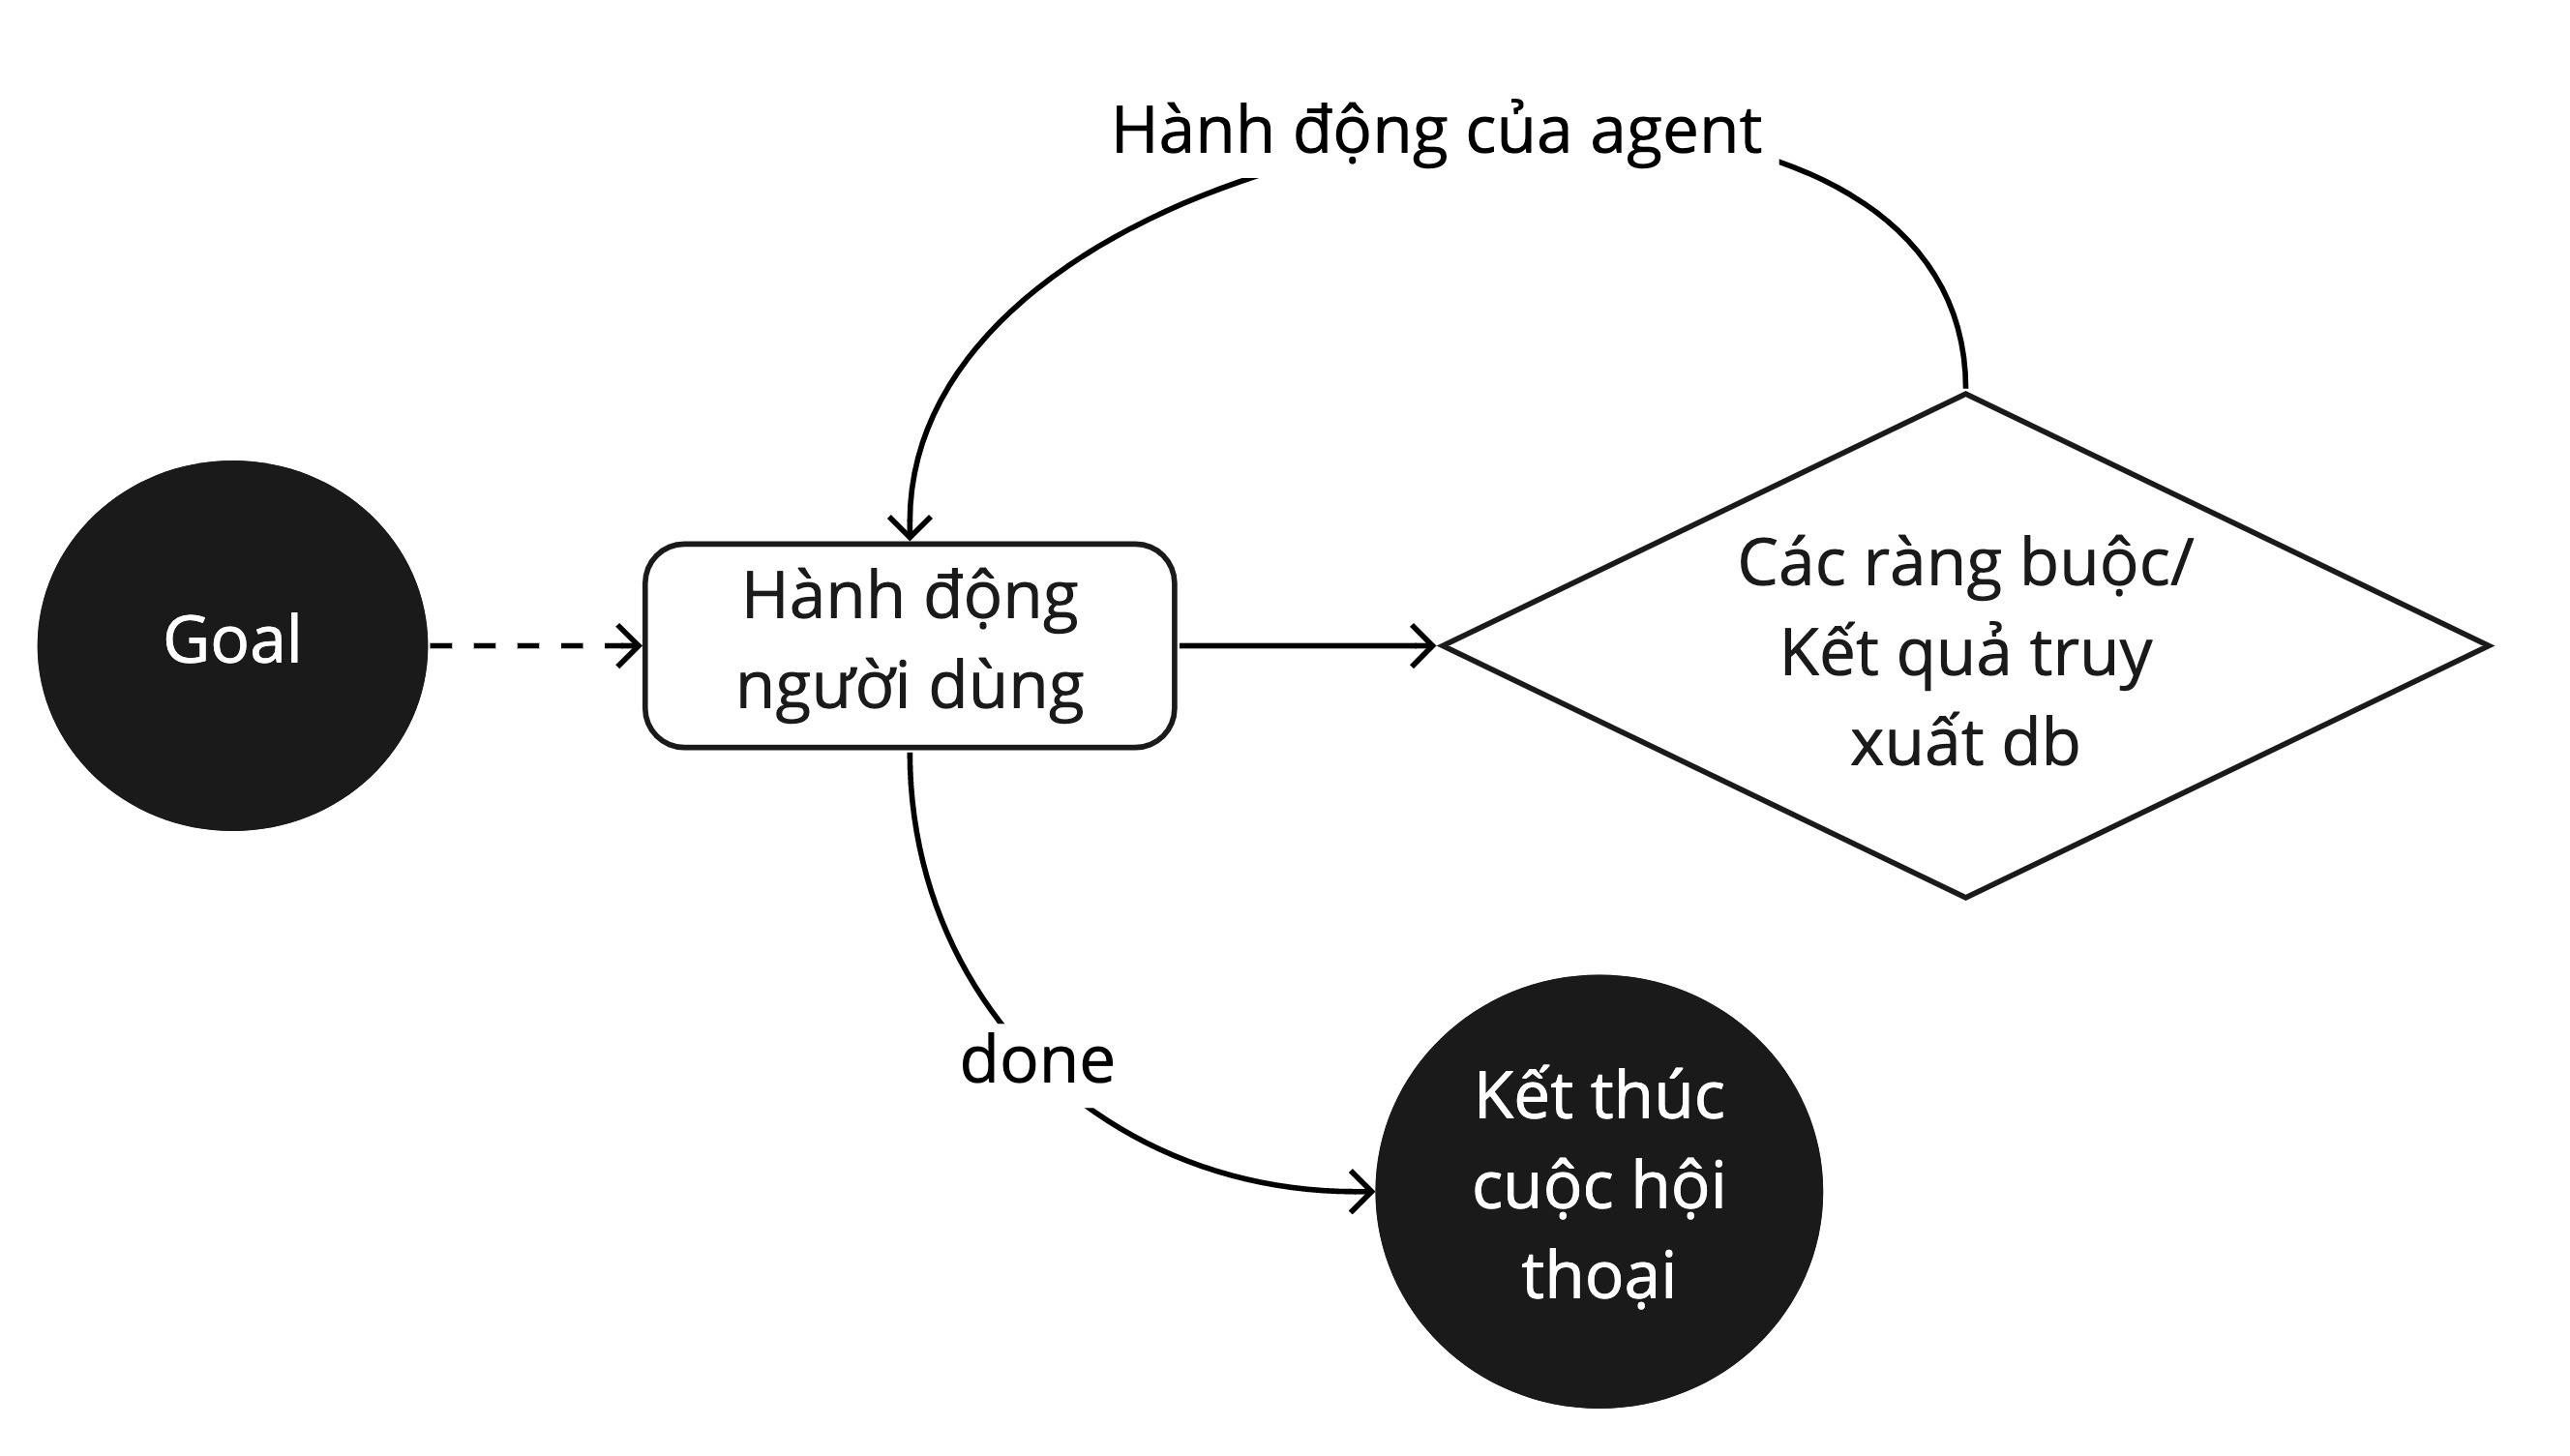
\includegraphics[scale=0.16]{thesis/chatbot/phuongphap/img/dialog.jpg}
    \caption{Sơ đồ biểu diễn tổng quát luật của hội thoại}
    \label{fig:dialog}
\end{figure}

Đầu tiên, ta xác định mục tiêu của người dùng trong hội thoại. Với
mục tiêu đó, lần lượt đưa ra các hành động tương ứng của người dùng,
qua mỗi lần nhận được hành động hệ thống sẽ kiểm tra các ràng buộc,
và trả về kết quả sau khi truy vấn lên cơ sở dữ liệu, tương ứng
đưa ra hành động cho tác nhân. Quá trình lặp lại cho đến khi
hoàn thành mục tiêu thì kết thúc hội thoại. Ví dụ một luật của
hội thoại cho mục tiêu yêu cầu giá bán sản phẩm có cấu trúc
như \ref{exam:rule}.

\renewcommand{\textboxenvname}{Ví dụ}
\begin{textbox}[exam:rule]{Luật của hội thoại cho mục tiêu yêu cầu giá bán sản phẩm}
\begin{Verbatim}[breaklines=true, breakanywhere=true]
"request_cost_product": [
    {
        "node": [
            {"id": 1, "intent": "request", "inform_slots": [], "request_slots": ["cost_product"]},
            {"id": 1, "intent": "request", "inform_slots": ["name_product"], "request_slots": ["cost_product"]},
            ...
        ],
        "condition": [
            {"id": 2, "rule": "exist", "entity": ["name_product"], "output": {"yes": 4, "no": 3}},
            ...
        ],
        "net": [
            {"Source": "start", "Destination": 1, "intent": "", "inform_slots": [], "request_slots": []},
            {"Source": 1, "Destination": 2, "intent": "check_condition", "inform_slots": [], "request_slots": []},
            ...
        ]
    }
]
\end{Verbatim}
\end{textbox}

\textit{Node} chứa các hành động của người dùng, gồm có \textit{id}
là số định danh hành động, \textit{intent} là ý định hành động
người dùng, và các danh sách chứa các thông tin yêu cầu hoặc
thông báo của người dùng. \textit{Condition} chứa các điều kiện
kiểm tra trạng thái hiện tại của hệ thống, và kết quả nhằm
điều hướng hành động kế tiếp. \textit{Net} chứa các hành động
của tác nhân hoặc tiến trình tiếp theo của hệ thống, gồm
\textit{source} chỉ điểm bắt đầu, \textit{destination} chỉ điểm đến,
\textit{intent} là ý định hành động của tác nhân hoặc chỉ hành vi
của hệ thống. Dựa trên bộ luật này, ta tạo ra các cuộc hội thoại có
cấu trúc như \ref{exam:dialog}, lần lượt là các hành động của
người dùng và tác nhân.

\renewcommand{\textboxenvname}{Ví dụ}
\begin{textbox}[exam:dialog]{Cuộc hội thoại được tạo bởi bộ luật}
\begin{Verbatim}[breaklines=true, breakanywhere=true]
[
    {"inform_slots": {}, "request_slots": {"cost_product": "UNK"}, "intent": "request", "speaker": "user"},
    {"intent": "request", "inform_slots": {}, "request_slots": {"name_product": "UNK"}, "speaker": "agent"},
    {"inform_slots": { "name_product": "dam hoa"}, "request_slots": {}, "intent": "inform", "speaker": "user"},
    {"intent": "inform", "inform_slots": {"cost_product": "160k"}, "request_slots": [], "speaker": "agent"},
    {"inform_slots": {}, "request_slots": {}, "intent": "ok", "speaker": "user"},
    {"intent": "match_found", "inform_slots": {}, "request_slots": {}, "speaker": "agent"},
    {"inform_slots": {}, "request_slots": {}, "intent": "ok", "speaker": "user"},
    {"intent": "done", "inform_slots": {}, "request_slots": {},"speaker": "agent"},
    {"inform_slots": {}, "request_slots": {}, "intent": "done", "speaker": "user"}
]
\end{Verbatim}
\end{textbox}

\subsubsection{Quá trình warmup}
Quá trình huấn luyện tác nhân trong giai đoạn warm-up được mô tả như
trong hình \ref{fig:warmupflow}.

\begin{figure}[ht!]
    \centering
    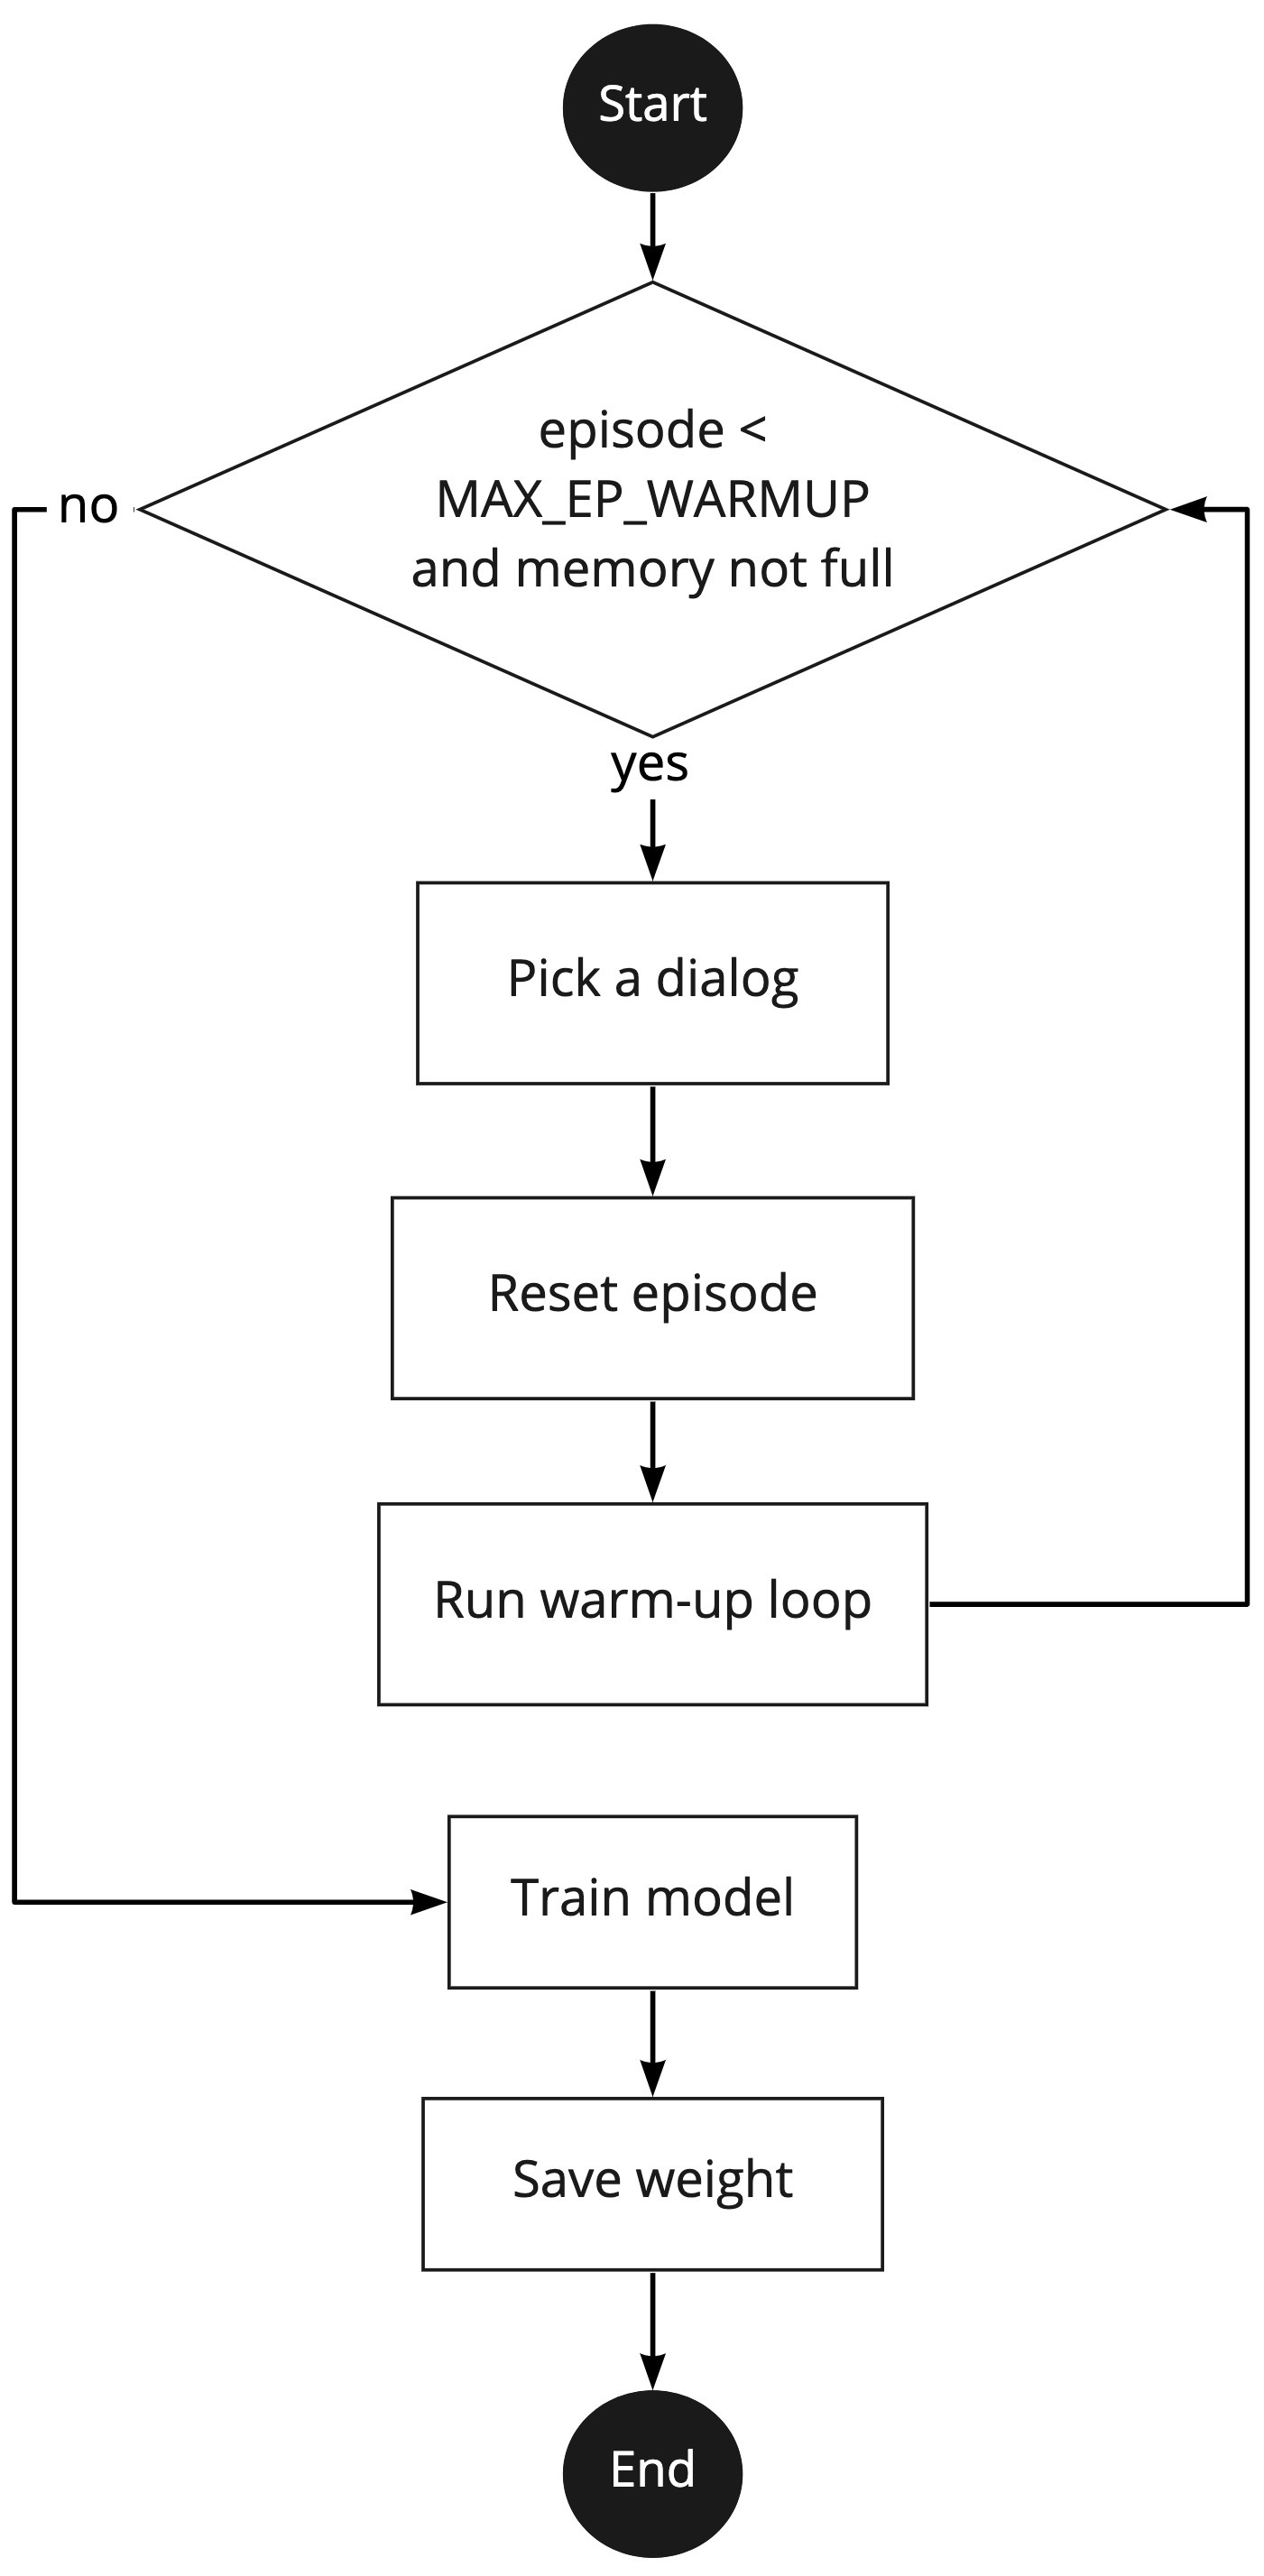
\includegraphics[scale=0.17]{thesis/chatbot/phuongphap/img/warmup_flow.jpg}
    \caption{Sơ đồ quá trình huấn luyện mô hình - giai đoạn warm-up}
    \label{fig:warmupflow}
\end{figure}

Đầu tiên, ta kiểm tra số lượt hội thoại hiện tại đã được thực hiện
không vượt quá số lượt lớn nhất chỉ định và bộ nhớ của tác nhân
còn trống. Kế tiếp, ta lấy một hội thoại (dialog) trong dữ liệu
các bộ hội thoại đã được tạo trước đó. Hội thoại này sẽ được
sử dụng cho các quyết định hành động sau này. Khởi tạo và thiết lập
lại toàn bộ thông tin của cuộc hội thoại như trạng thái, hành động
của người dùng, tác nhân, ... Trong đó, ta có khởi tạo hành động
đầu tiên của người dùng, ở đây là lấy hành động đầu tiên trong
hội thoại và gửi nó đến bộ quản lý trạng thái hội thoại. Sau đó
thực hiện vòng lặp warm-up được mô tả cụ thể ở hình
\ref{fig:warmup}. Sau khi hoàn tất quá trình khởi tạo ký ức cho
tác nhân, ta sẽ mang toàn bộ ký ức này đem đi huấn luyện cho
mô hình mạng nơ-ron sẽ được trình bày ở phần \ref{subsec:agent}.

Hình \ref{fig:warmup} mô tả một vòng lặp warm-up.

\begin{figure}[ht!]
    \centering
    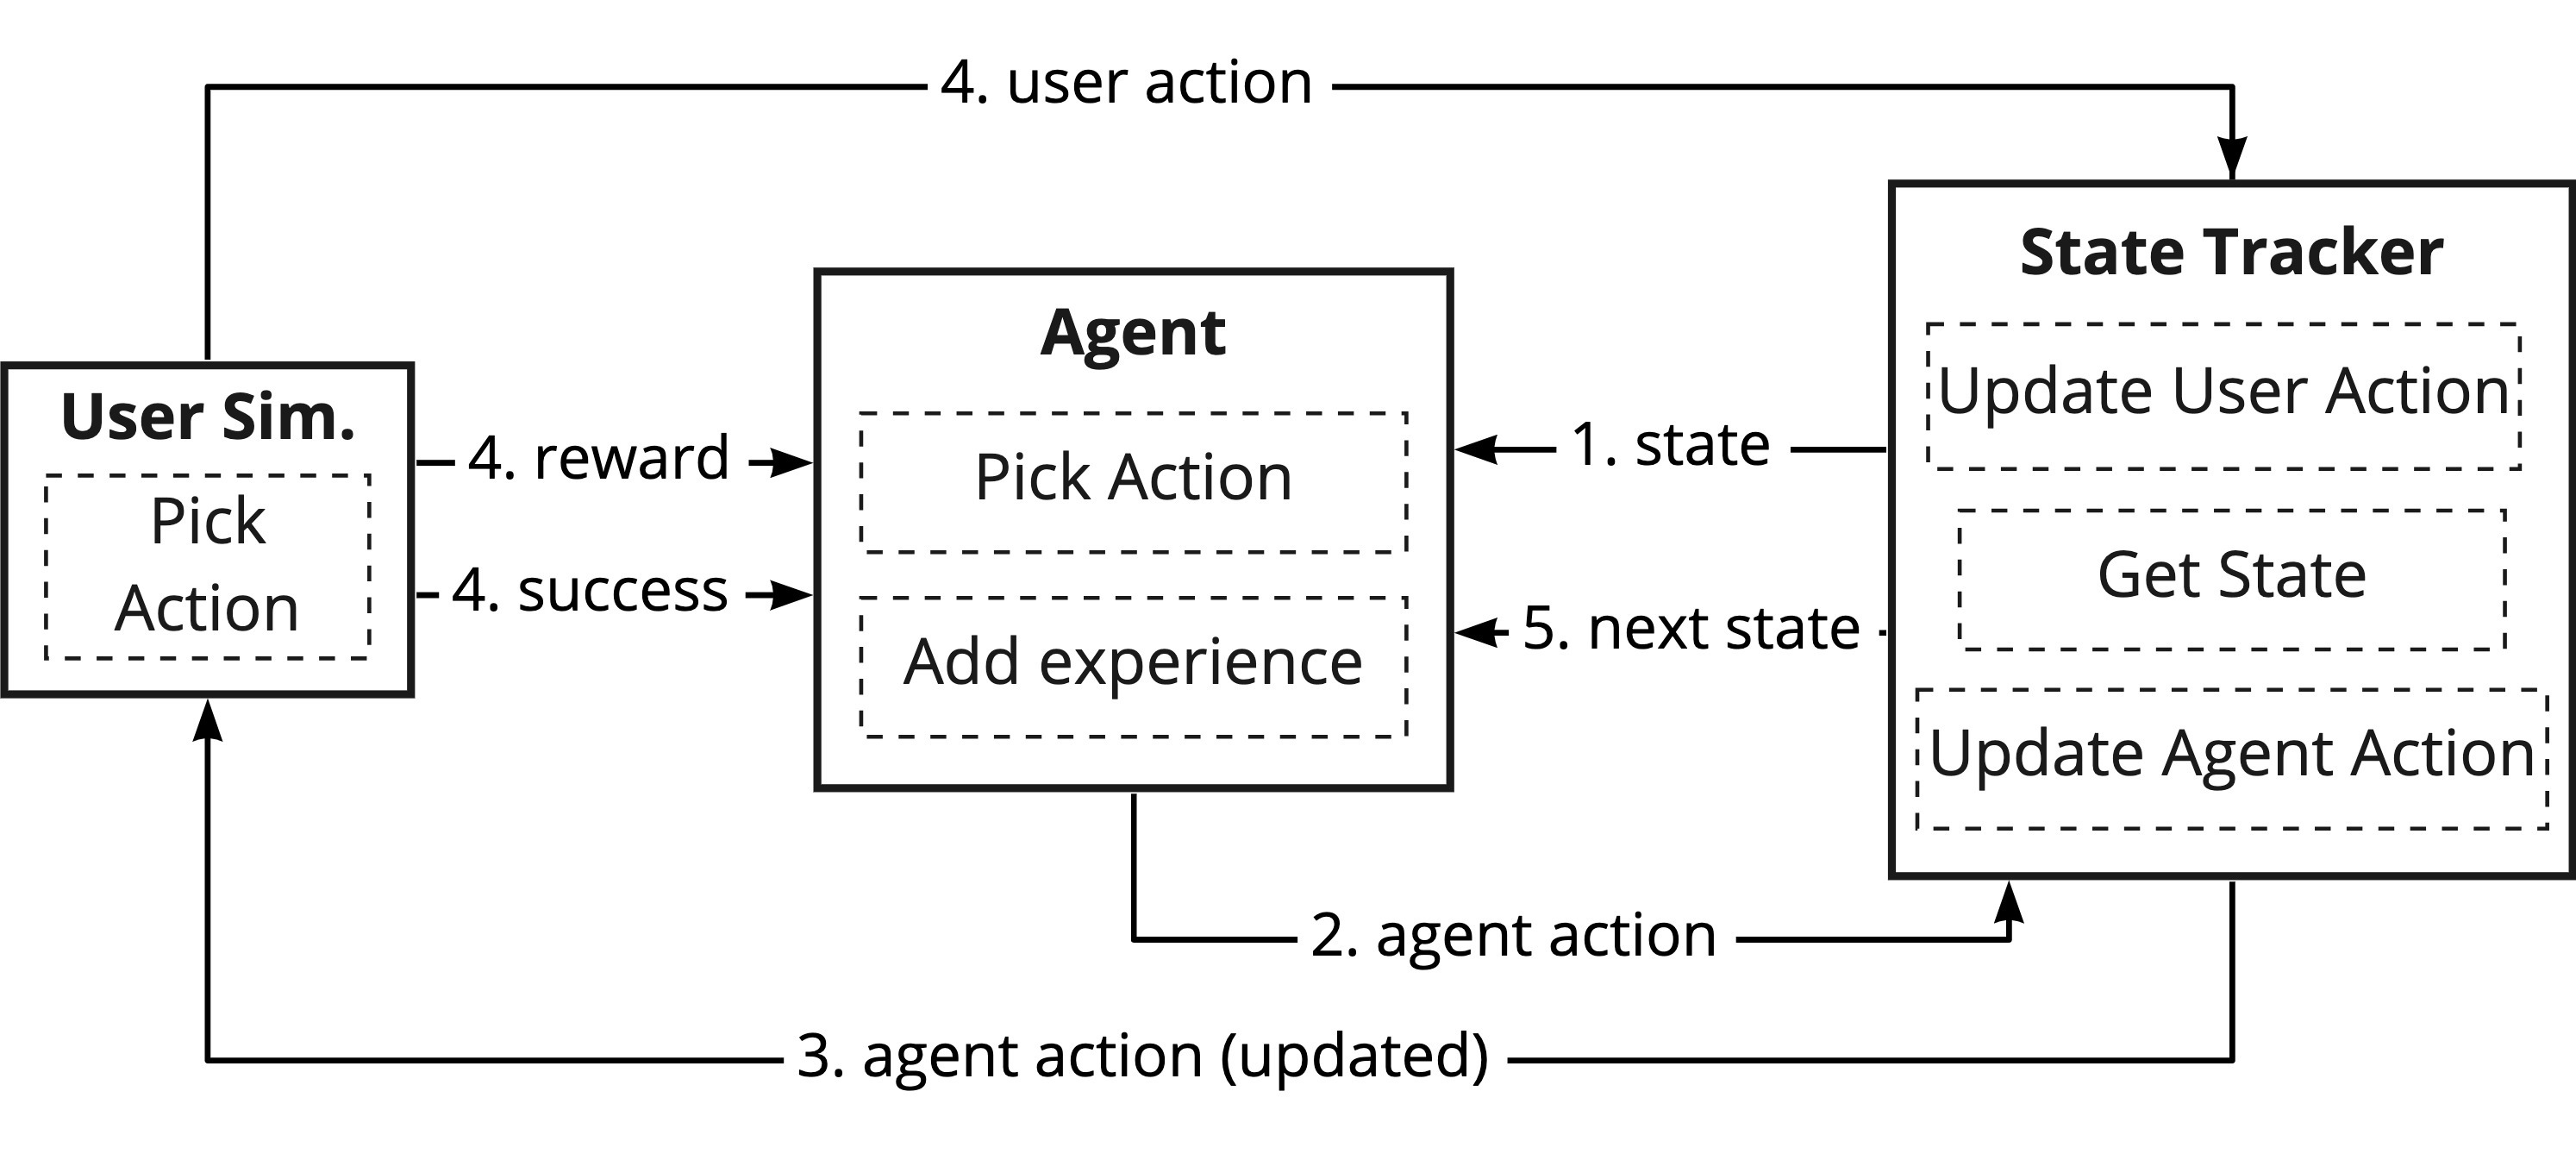
\includegraphics[scale=0.14]{thesis/chatbot/phuongphap/img/warmup.jpg}
    \caption{Vòng lặp huấn luyện - giai đoạn warm-up}
    \label{fig:warmup}
\end{figure}

Mỗi một vòng thực hiện là một lượt đối thoại qua lại giữa người dùng
và tác nhân. Cụ thể:

\begin{itemize}
    \item \textbf{Bước 1:} Ta lấy ra \textit{state} - trạng thái
    hiện tại của hội thoại từ \textit{State Tracker} - bộ quản lý
    trạng thái hội thoại, trạng thái này có thể là trạng thái
    khởi tạo nếu như vừa bắt đầu hội thoại hoặc là trạng thái của
    toàn bộ cuộc hội thoại giữa người dùng và tác nhân. Mục đích lấy
    trạng thái ở giai đoạn này là để ghi vào bộ nhớ, và sẽ làm
    dữ liệu đầu vào (input) cho việc huấn luyện mô hình sau này.
    \item \textbf{Bước 2:} Tác nhân sau khi nhận được input từ
    bước trước sẽ lưu vào kí ức (experience) của nó và lấy ra một
    \textit{action} (hành động) từ trong \textit{dialog} và gửi
    ngược về lại bộ quản lý trạng thái hội thoại. Ở đây, nó sẽ được
    bộ quản lý trạng thái hội thoại cập nhật số lượt đã được
    thực hiện trong hội thoại. Đồng thời bộ quản lý trạng thái
    hội thoại cũng sẽ cập nhật lại trạng thái của hội thoại.
    \item \textbf{Bước 3:} Hành động sau khi được cập nhật đầy đủ
    thông tin sẽ được gửi cho \textit{User Simulator} - bộ
    mô phỏng người dùng. Bộ mô phỏng người dùng cũng dựa vào
    \textit{dialog}, lấy ra một hành động, đồng thời sẽ dựa vào
    các luật đã được quy định trước để chấm \textit{reward}
    (điểm thưởng) và tín hiệu success (thành công) để giúp tác nhân
    có thể tự điều chỉnh hành vi để học. Ở đây, tác nhân cũng sẽ
    ghi lại toàn bộ vào ký ức của nó.
    \item \textbf{Bước 4:} Hành động của người dùng ở bước trước sẽ
    tiếp tục được gửi đi đến bộ quản lý trạng thái hội thoại và
    được cập nhật thông tin cụ thể tương tự ở bước 2. Đồng thời
    bộ quản lý trạng thái hội thoại cũng cập nhật trạng thái của nó.
    \item \textbf{Bước 5:} Trạng thái tiếp theo được lấy từ bộ
    quản lý trạng thái hội thoại và quay lại giống bước 1.
\end{itemize}

Quá trình này sẽ được thực hiện liên tục cho đến khi thực thi
lần lượt hết tất cả các hành động của người dùng và
tác nhân trong \textit{dialog}.

\subsubsection{Ví dụ}
Như trình bày ở trên, trong giai đoạn warm-up, ta sẽ lấy một đoạn
hội thoại được tạo sẵn. Xét mẫu hội thoại như ví dụ
\ref{exam:dialog3}. Giả sử, trạng thái chỉ chứa các ý định hành động
hiện tại của người dùng lần lượt là: hello, inform, request, reject,
done. Ta mã hóa về dạng one-hot vec-tơ để làm đầu vào cho mạng
nơ-ron. Quá trình huấn luyện trong giai đoạn warm-up như sau:

\begin{itemize}
    \item Đầu tiên, bộ mô phỏng người dùng sẽ lấy hành động đầu tiên
    trong hội thoại là yêu cầu thông tin màu sắc (request(cost\_product)).
    Sau đó nó được gửi tới bộ quản lý trạng thái hội thoại. Bộ quản lý
    trạng thái hội thoại sẽ thêm thông tin số lượt thực hiện là 1 vào
    hành động của người dùng để kiểm soát hội thoại kéo dài không quá
    số lượt cho phép (20). Đồng thời lấy trạng thái hiện tại của hội thoại
    gửi qua cho tác nhân là $[0\; 0\; 1\; 0\; 0]$. Quá trình được
    biểu diễn như hình \ref{fig:examwarmup}.
\end{itemize}

\begin{figure}[ht!]
    \centering
    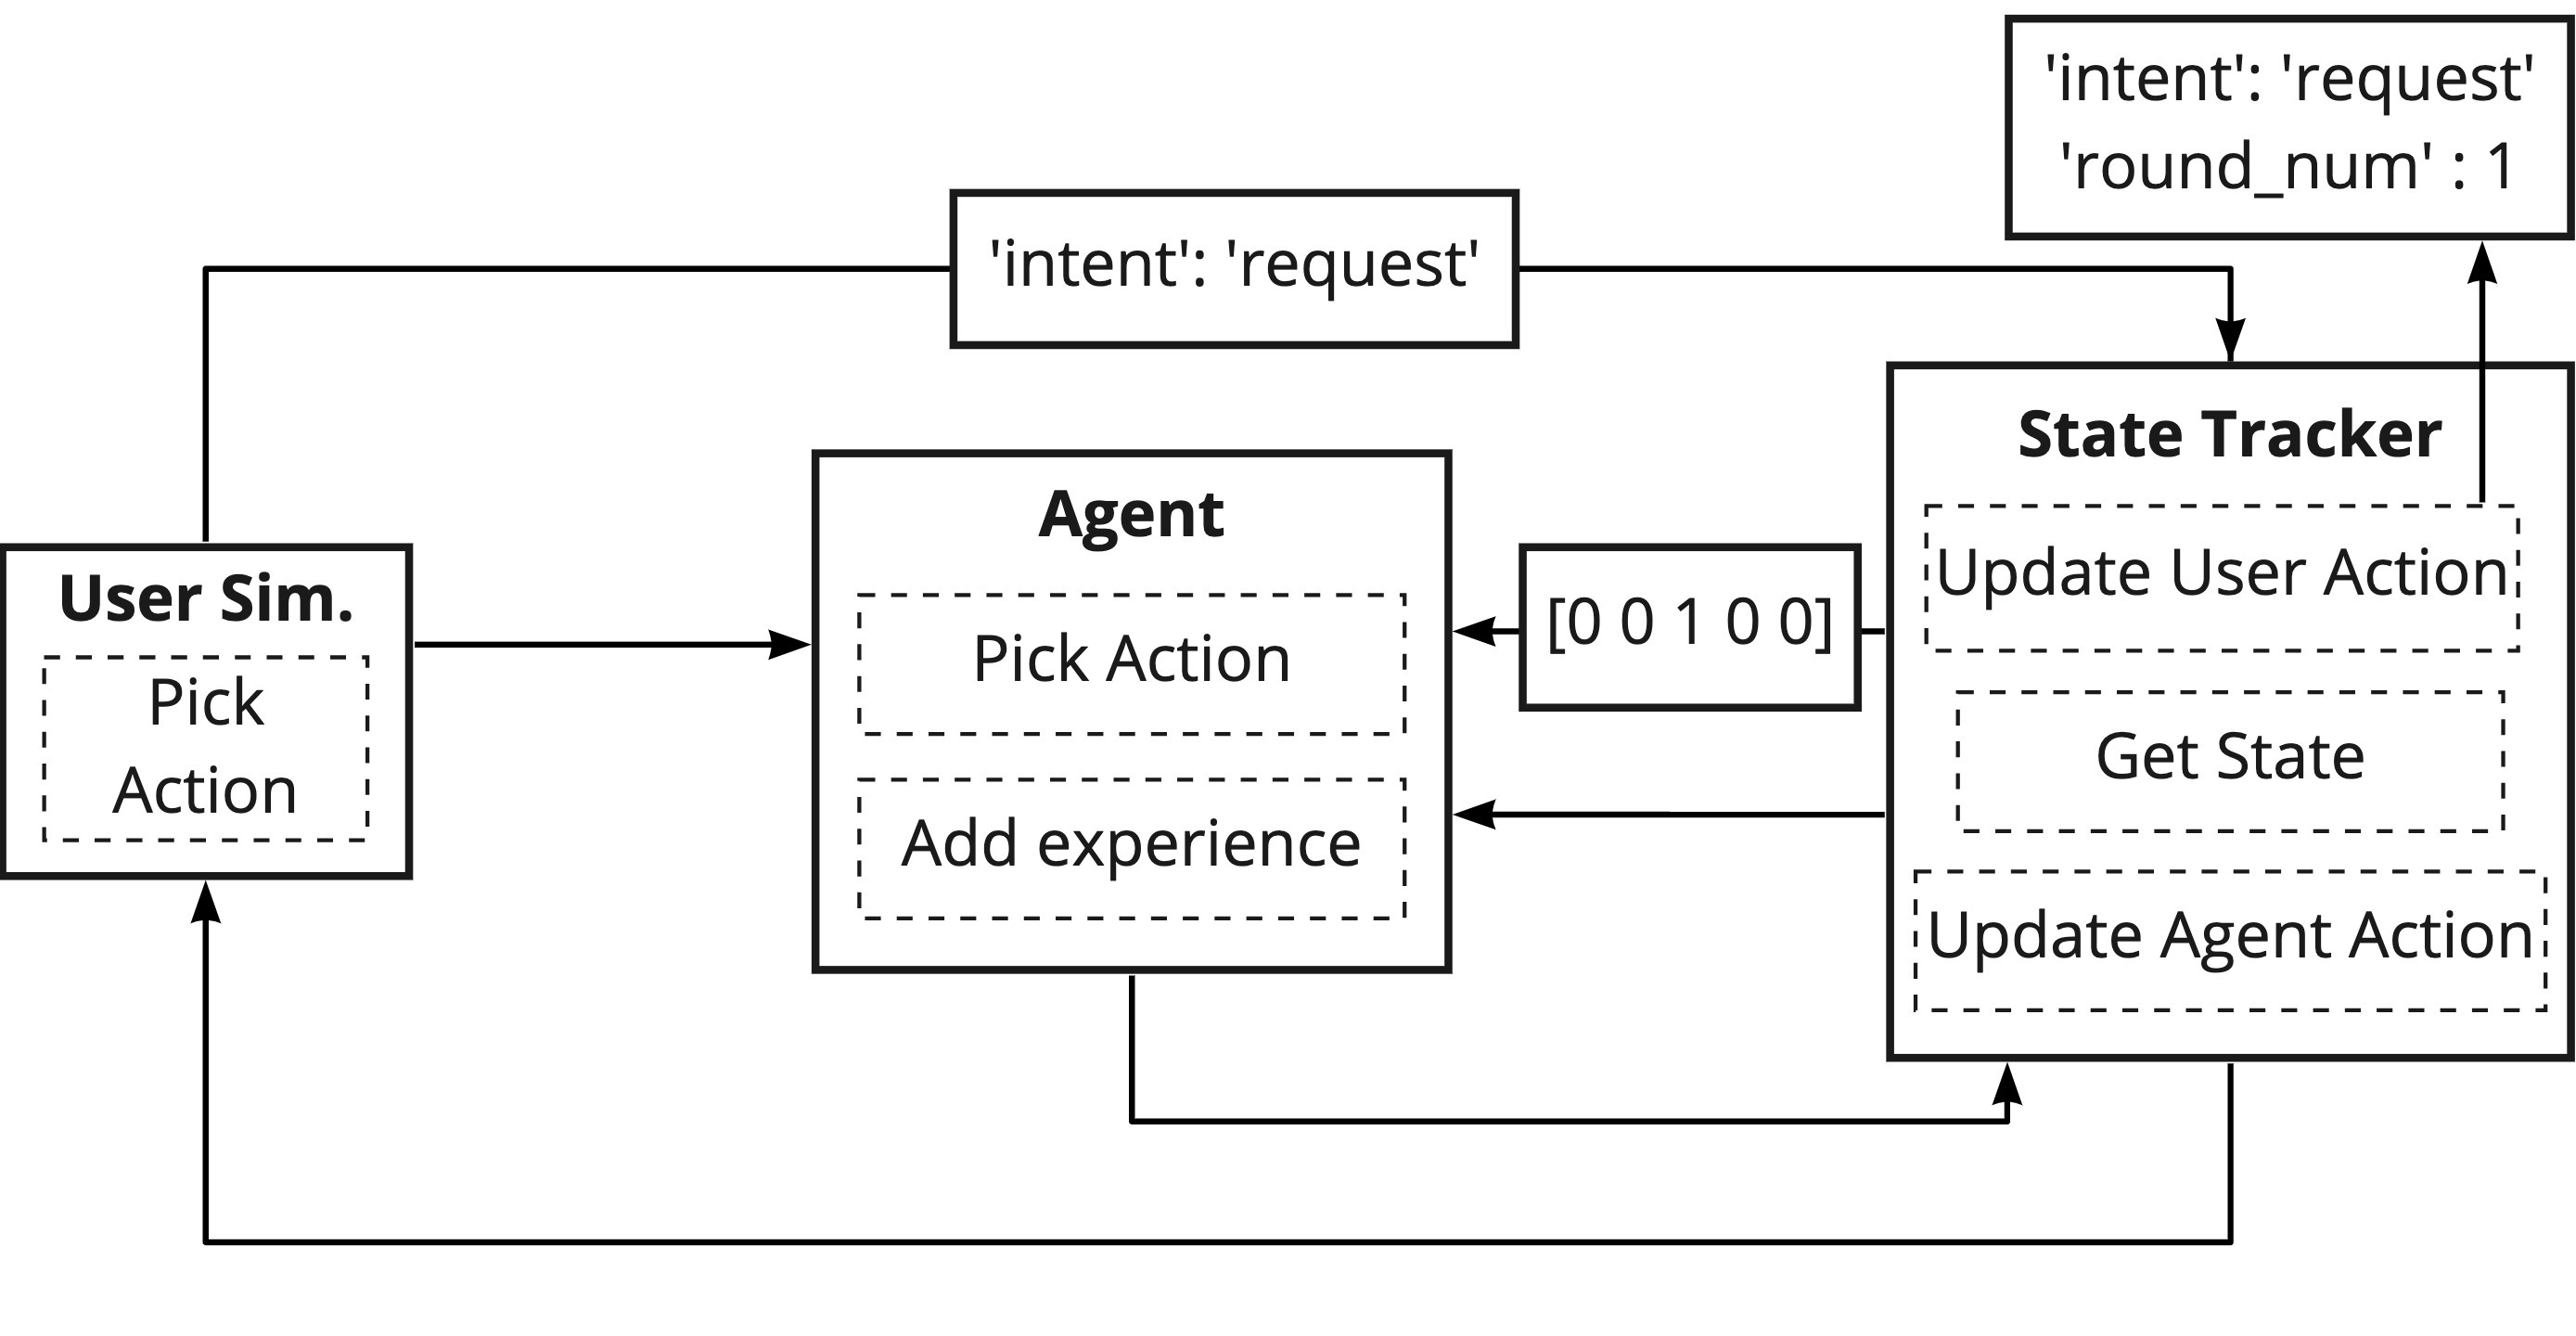
\includegraphics[scale=0.15]{thesis/chatbot/phuongphap/img/warmup_exam.jpg}
    \caption{Ví dụ quá trình huấn luyện bước 1 - giai đoạn warm-up}
    \label{fig:examwarmup}
\end{figure}

\begin{itemize}
    \item Tại đây, tác nhân sẽ lấy hành động kế tiếp trong hội thoại
    là yêu cầu tên sản phẩm (request(name\_product)). Sau đó nó được
    gửi tới bộ quản lý trạng thái hội thoại. Tương tự, bộ quản lý
    trạng thái hội thoại sẽ thêm thông tin số lượt thực hiện vào
    hành động của tác nhân là 1 và gửi qua cho bộ mô phỏng người dùng.
    Quá trình được biểu diễn như hình \ref{fig:examwarmup1}.
\end{itemize}

\begin{figure}[ht!]
    \centering
    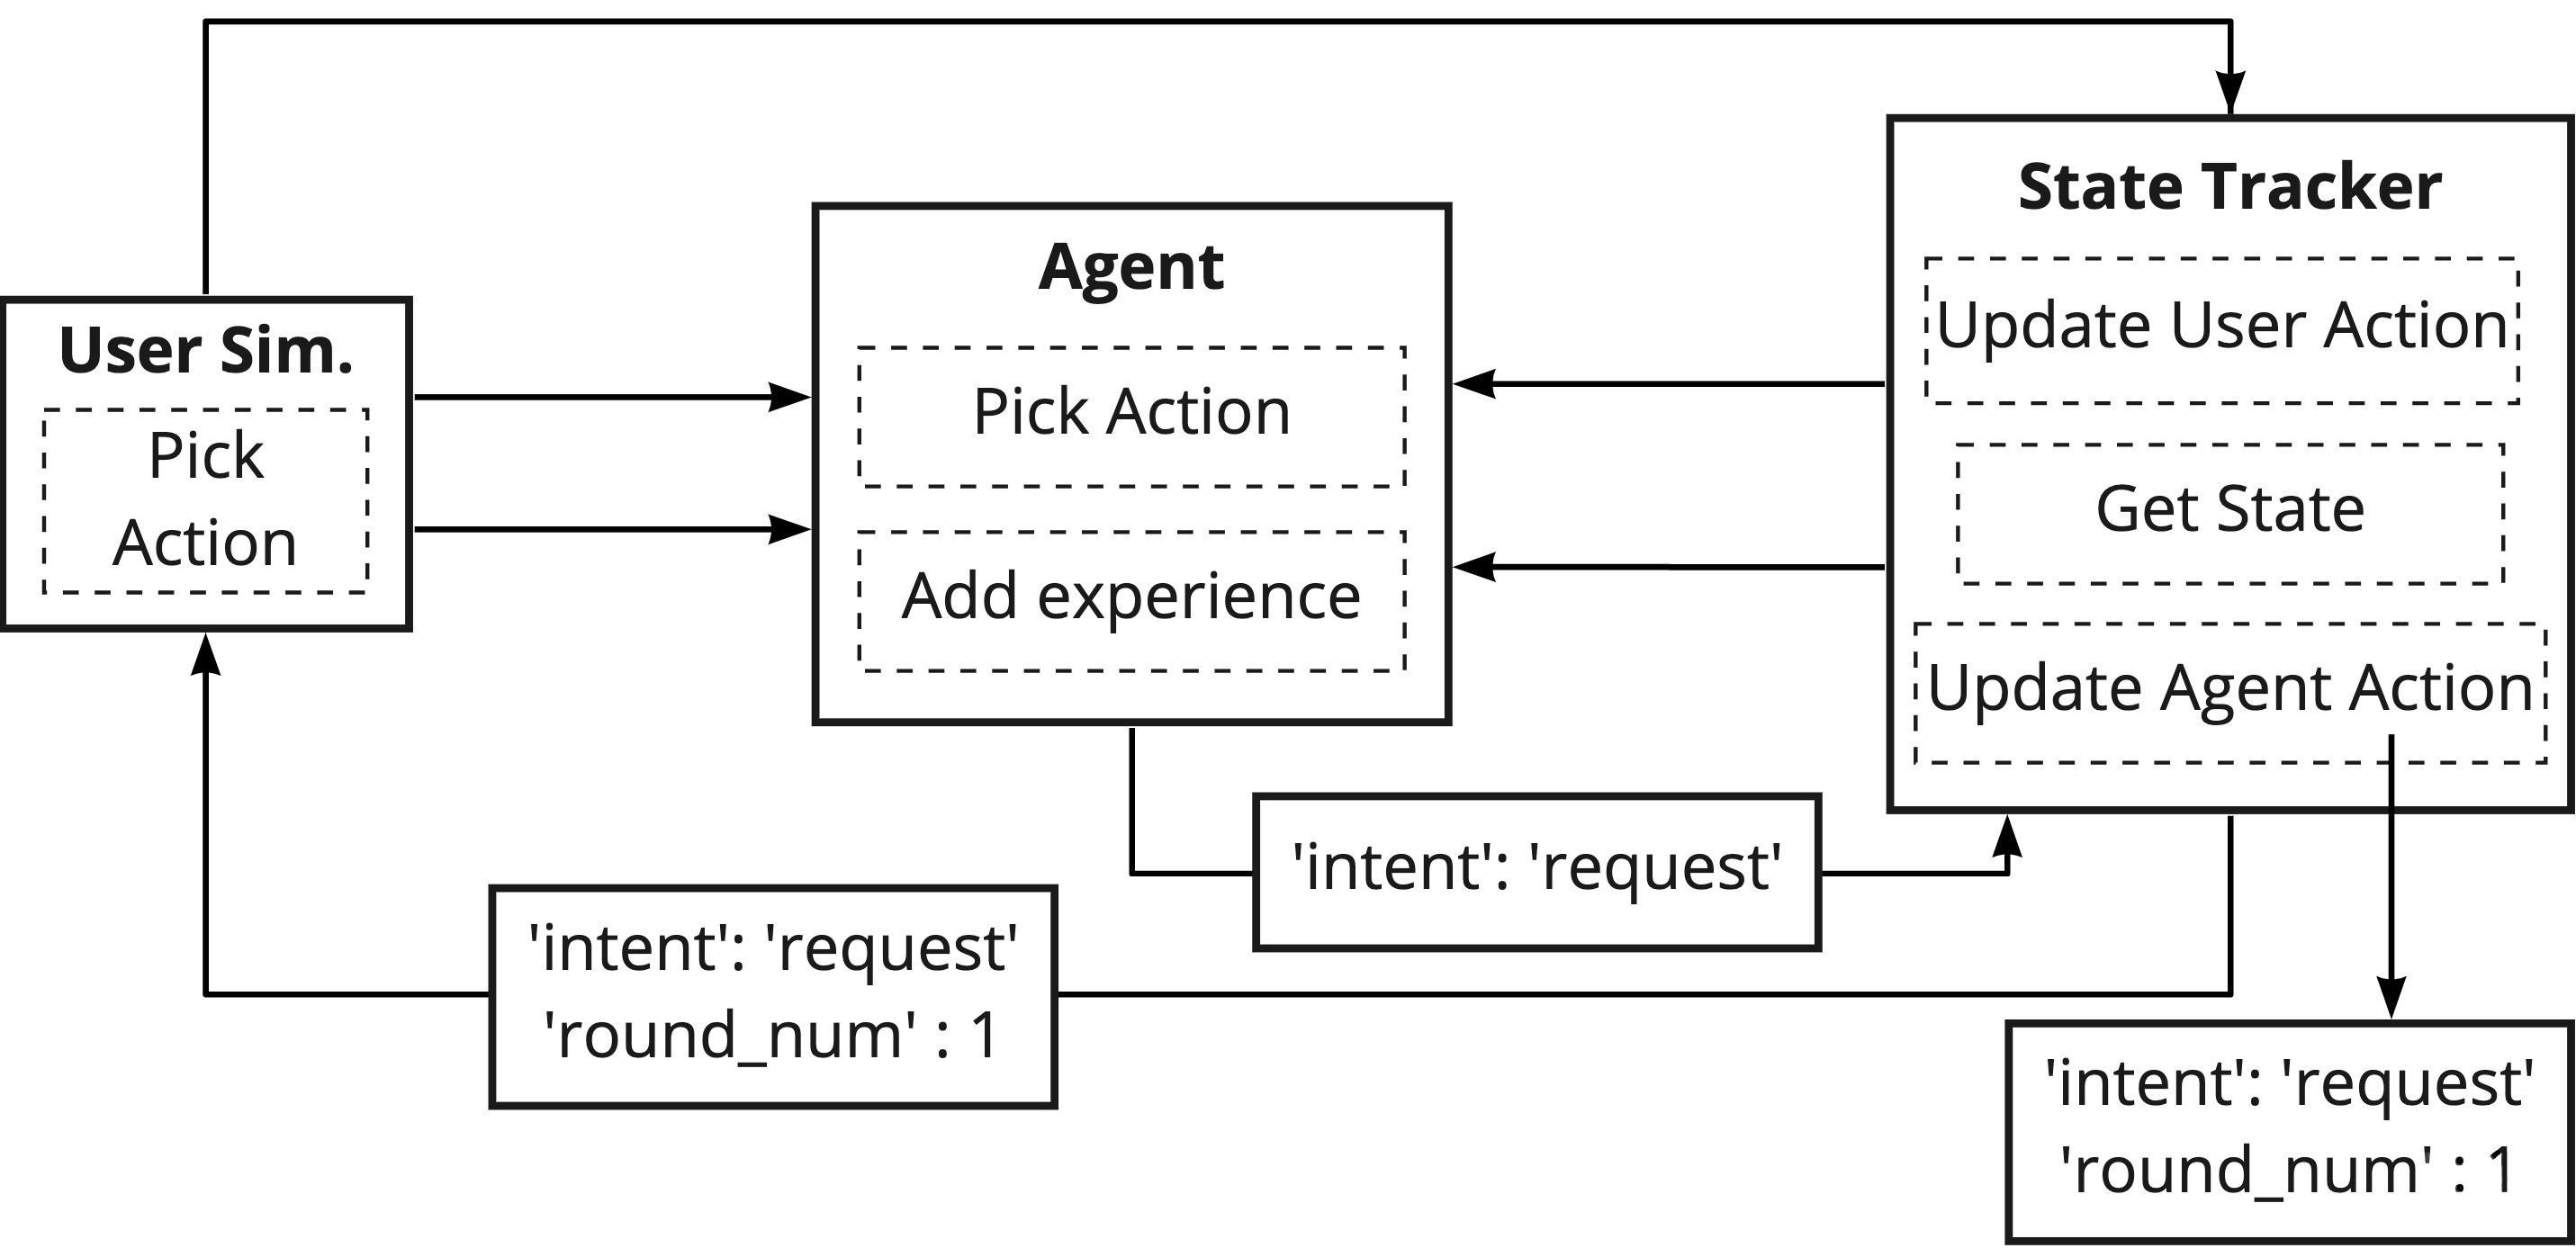
\includegraphics[scale=0.15]{thesis/chatbot/phuongphap/img/warmup_exam1.jpeg}
    \caption{Ví dụ quá trình huấn luyện bước 2 - giai đoạn warm-up}
    \label{fig:examwarmup1}
\end{figure}

\begin{itemize}
    \item Tương tự, bộ mô phỏng người dùng sẽ lấy hành động kế tiếp
    trong hội thoại là thông báo tên sản phẩm (inform(name\_product)).
    Gửi tới bộ quản lý trạng thái hội thoại. Bộ quản lý trạng thái
    hội thoại sẽ thêm thông tin số lượt vào hành động của người dùng
    là 2. Cập nhật và lấy trạng thái hiện tại của hội thoại gửi qua
    cho tác nhân là $[0\; 1\; 0\; 0\; 0]$. Ngoài ra, bộ mô phỏng
    người dùng cũng sẽ gửi điểm thưởng cho phản hồi vừa rồi của
    tác nhân (request(name\_product)). Với cách cho điểm thưởng như
    được mô tả ở mục \ref{subsec:reward}. Ta giả sử, điểm thưởng là
    -1. Quá trình được biểu diễn như hình \ref{fig:examwarmup2}.
\end{itemize}

\begin{figure}[ht!]
    \centering
    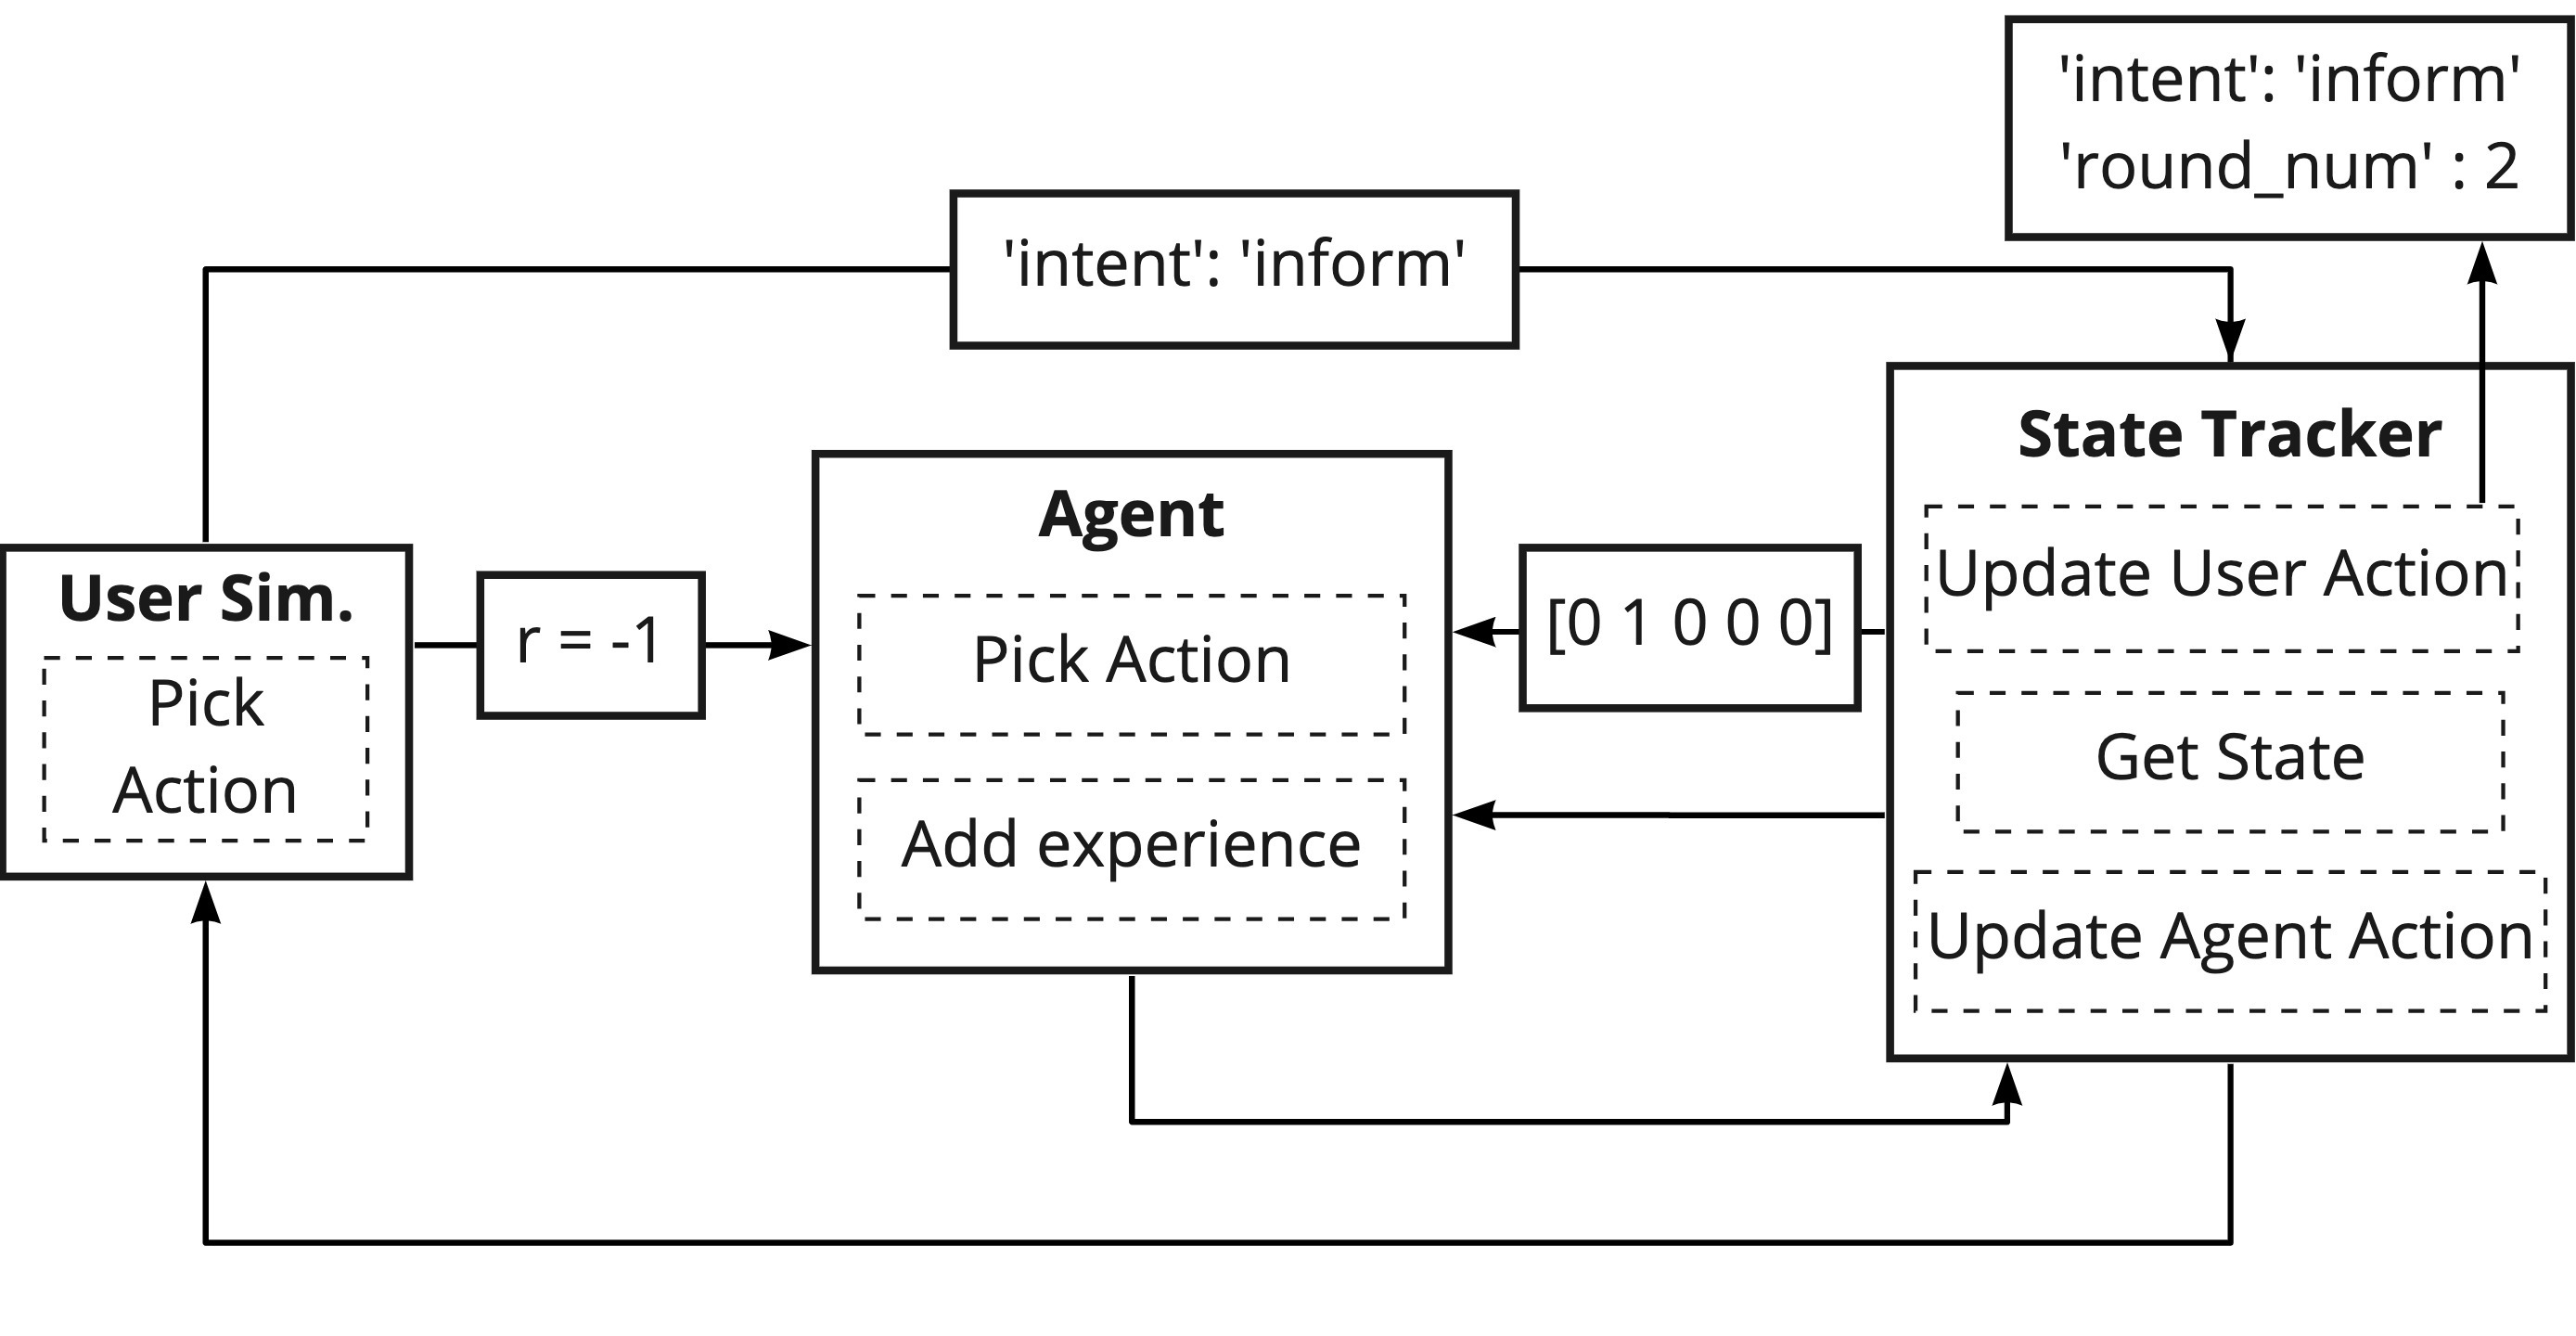
\includegraphics[scale=0.15]{thesis/chatbot/phuongphap/img/warmup_exam2.jpg}
    \caption{Ví dụ quá trình huấn luyện bước 3, 4 và 5 - giai đoạn warm-up}
    \label{fig:examwarmup2}
\end{figure}

Trạng thái hội thoại tại thời điểm này chính là trạng thái kế tiếp
của hành động trước đó (request(cost\_product)) của người dùng.

Tại đây, chúng ta đã có đầy đủ thông tin:
\begin{itemize}
    \item State ($s$): trạng thái hiện tại khi người dùng yêu cầu
    thông tin (request(cost\_product)) là $[0\; 0\; 1\; 0\; 0]$.
    \item Next state ($s'$): trạng thái kế tiếp của người dùng
    sau khi tác nhân phản hồi yêu cầu tên sản phẩm
    (request(name\_product)) là $[0\; 1\; 0\; 0\; 0]$.
    \item Action ($a$): hành động tác nhân phản hồi tại
    trạng thái $s$ là request(name\_product).
    \item Reward ($r_0$): phần thưởng cho hành động $a$ là -1
\end{itemize}

Toàn bộ thông tin này được lưu vào bộ nhớ. Sau khi quá trình
ghi nhớ các hội thoại mẫu này kết thúc. Ta sẽ thực hiện việc
huấn luyện như mô tả ở mục \ref{subsec:deepqlearning}

\subsection{Giai đoạn huấn luyện (Training stage)}

\subsubsection{Mục tiêu}
Đây là quá trình chính nhằm mục đích huấn luyện cho tác nhân có
khả năng thực hiện các hành động tương tự như con người, có
khả năng đáp trả giúp người dùng hoàn thành được mục tiêu khi
tham gia cuộc hội thoại. Quá trình huấn luyện sử dụng tập dữ liệu
\textit{User Goal}, chứa các mục tiêu của người dùng làm đầu vào
cho bộ mô phỏng người dùng. Dựa vào mục tiêu trên, bộ mô phỏng
người dùng tự đưa ra các hành động phù hợp. Tác nhân với kí ức trước
đã được học ở giai đoạn warm-up, đưa ra hành động phản hồi và
được huấn luyện lại sau một số lượt hội thoại diễn ra.

\subsubsection{Quá trình training}
Quá trình huấn luyện tác nhân trong giai đoạn training được mô tả
như trong hình \ref{fig:trainingflow}

\begin{figure}[!ht]
    \centering
    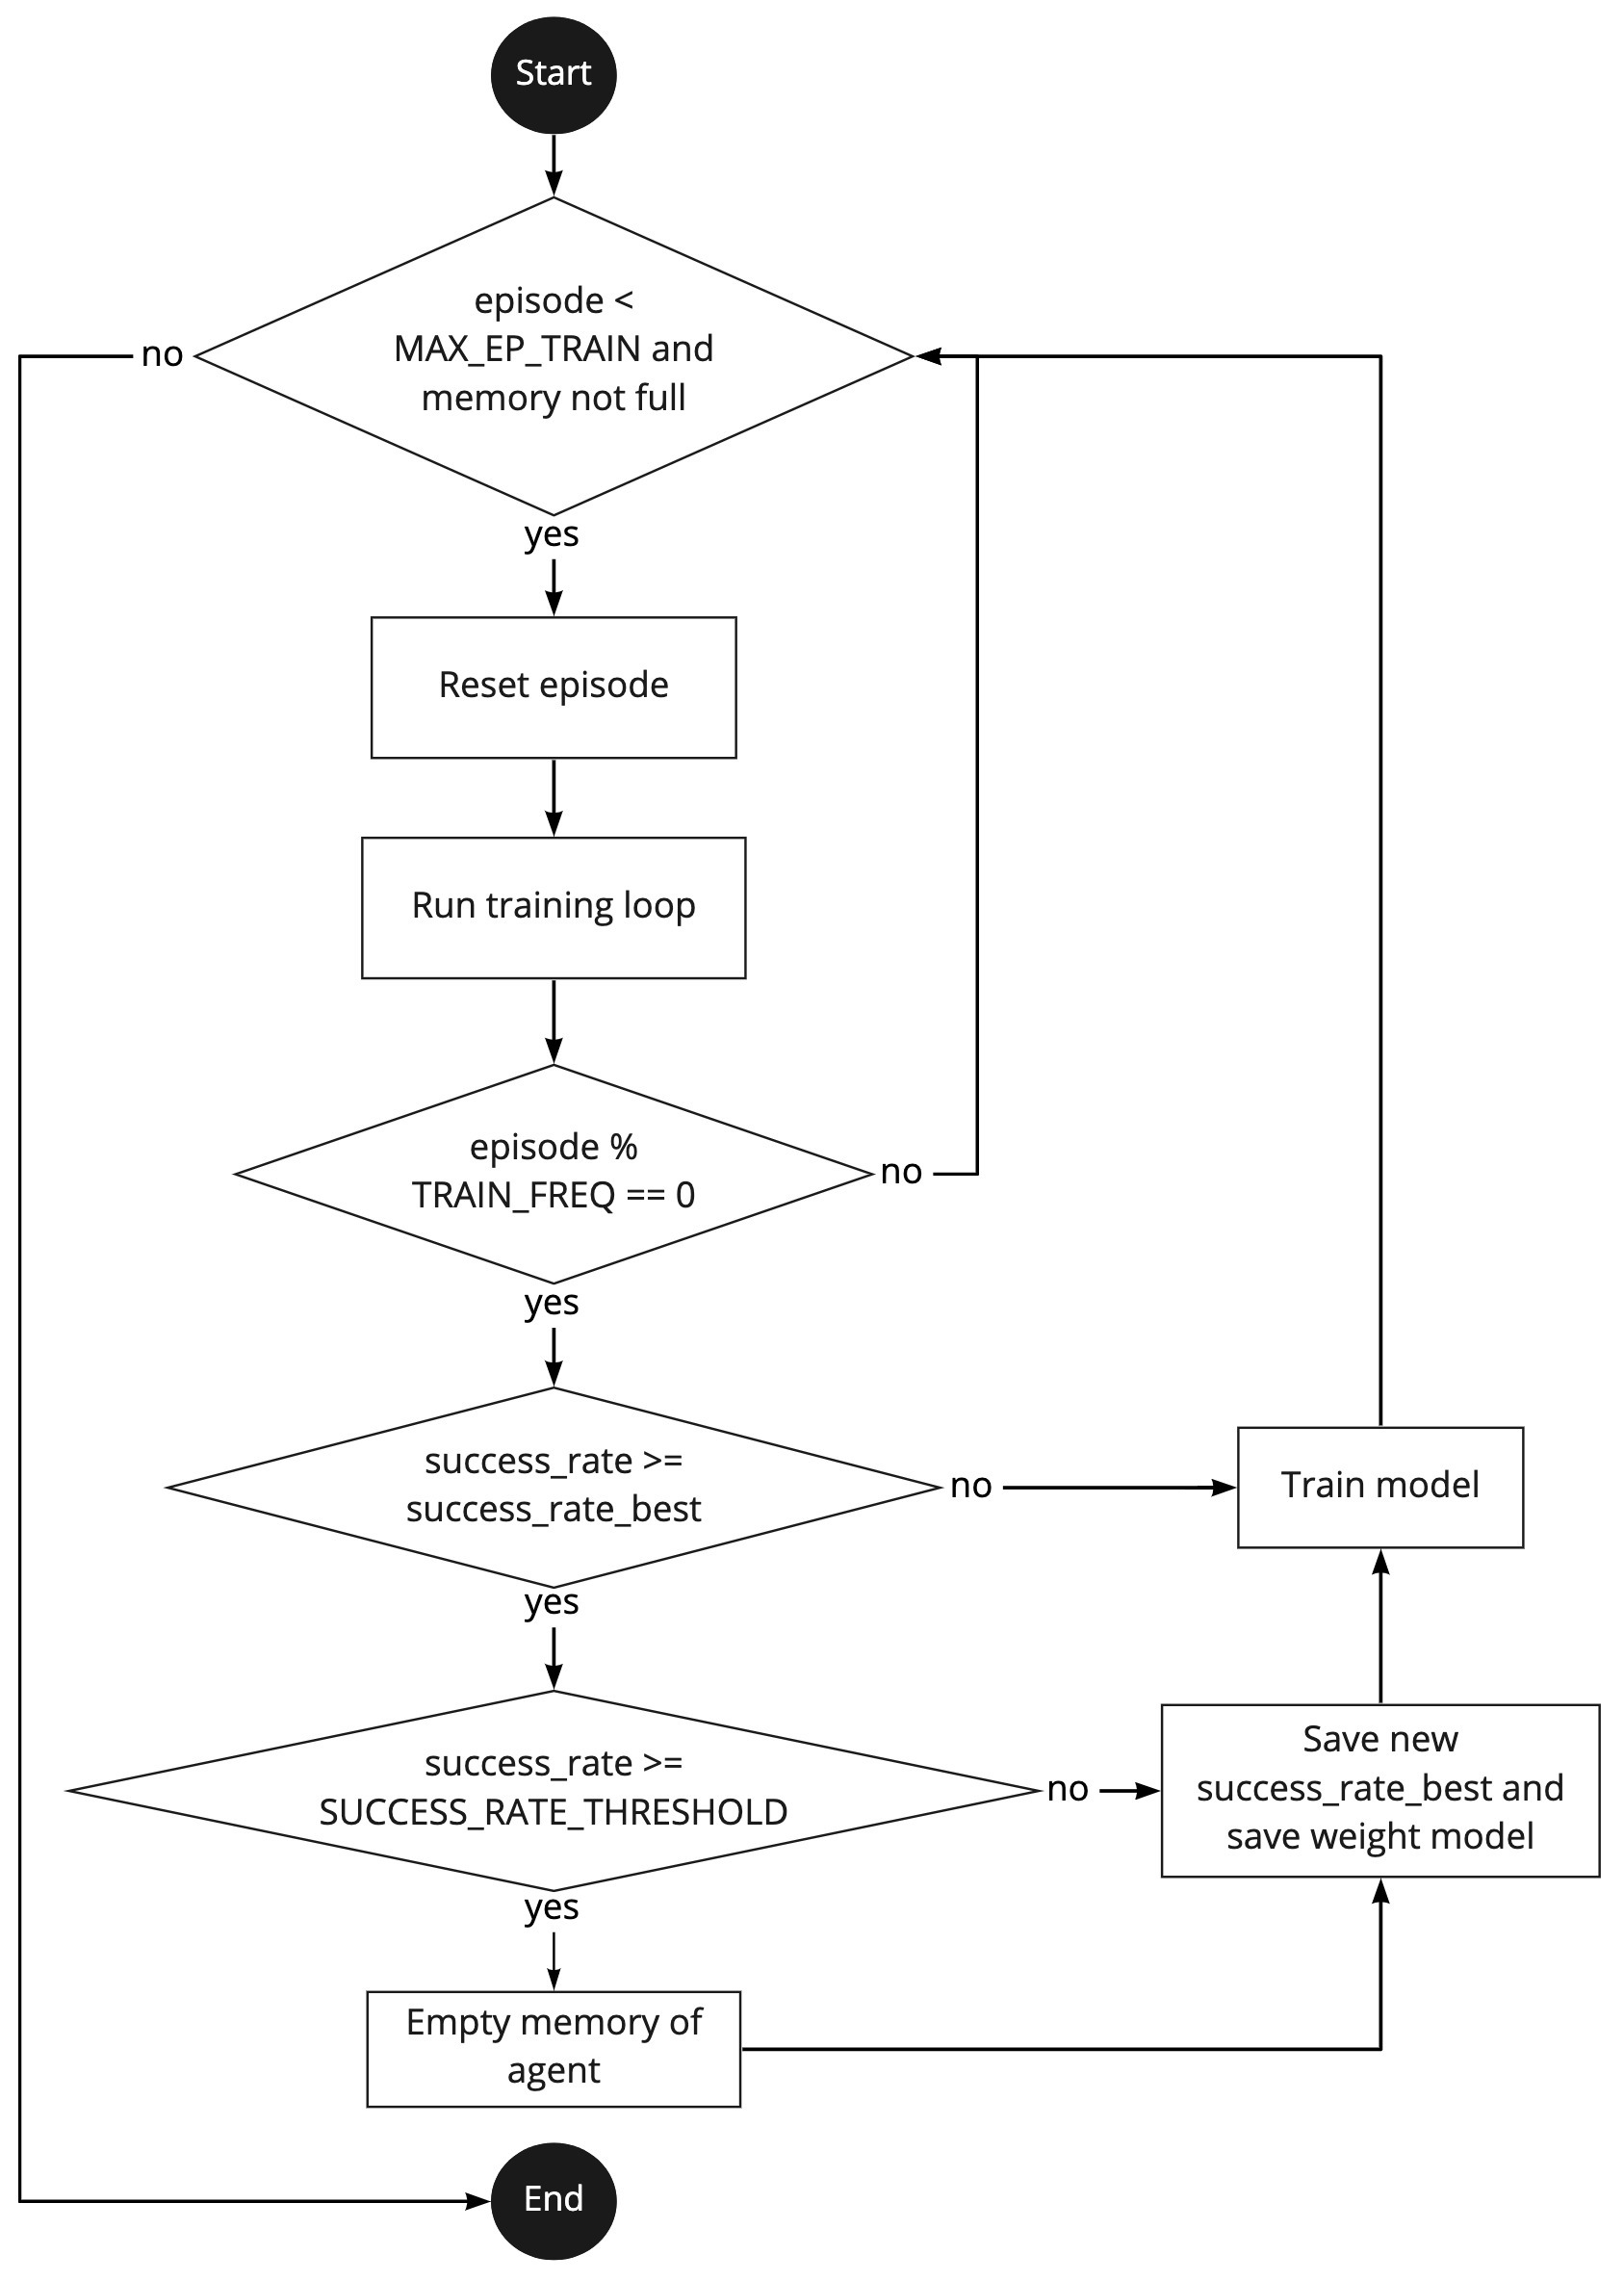
\includegraphics[scale=0.24]{thesis/chatbot/phuongphap/img/training_flow.jpg}
    \caption{Sơ đồ quá trình huấn luyện mô hình - giai đoạn training}
    \label{fig:trainingflow}
\end{figure}

Đầu tiên, giống với giai đoạn warm-up, ta kiểm tra số lượt hội thoại
hiện tại đã được thực hiện không vượt quá số lượt lớn nhất chỉ định
và bộ nhớ của tác nhân còn trống. Kế tiếp, quá trình khởi tạo và
thiết lập lại toàn bộ thông tin của cuộc hội thoại được thực hiện như
xóa lịch sử trạng thái, hành động của người dùng, tác nhân, ...
Tại bước này, bộ mô phỏng người dùng đồng thời lấy một mục tiêu
người dùng trong cơ sở dữ liệu, tạo ra hành động đầu tiên trong
cuộc hội thoại và lấy nó làm mục tiêu trong suốt cuộc hội thoại
diễn ra. Sau đó, là quá trình thực hiện vòng lặp training cho đến khi
kết thúc cuộc hội thoại. Vòng lặp này sẽ được mô tả cụ thể ở hình
\ref{fig:training}. Vòng lặp sẽ kết thúc sau mỗi lần cuộc hội thoại
được hoàn thành (thành công hoặc thất bại). Cứ mỗi một số hội thoại
nhất định được hoàn thành (được xác định bởi tham số
\textit{TRAIN\_FREQ}), ta kiểm tra tỉ lệ thành công trong số các
cuộc hội thoại đó. Nếu hiện tại là lớn nhất và lớn hơn một mức ngưỡng
cho trước thì xóa đi toàn bộ ký ức của tác nhân. Việc này nhằm
mục đích để tác nhân loại bỏ đi các trải nghiệm cũ, khi mà những
trải nghiệm đó đưa ra những quyết định không tốt, thì tốt hơn hết
chúng ta sẽ huấn luyện nó với phiên bản tốt hơn. Nếu không ta vẫn
giữ lại các ký ức đó và lưu lại tỉ lệ thành công tốt nhất và trọng số
của mô hình. Ở đây, ta có một tác nhân được huấn luyện với trạng thái
tốt nhất hiện tại. Nếu tỉ lệ thành công hiện tại không lớn nhất,
thì ta chỉ tiếp tục huấn luyện mô hình với những ký ức đang có.
Quá trình huấn luyện này sẽ kết thúc cho đến khi hết số lượt hội thoại
cần huấn luyện.

Hình \ref{fig:training} mô tả một vòng lặp training.

\begin{figure}[ht!]
    \centering
    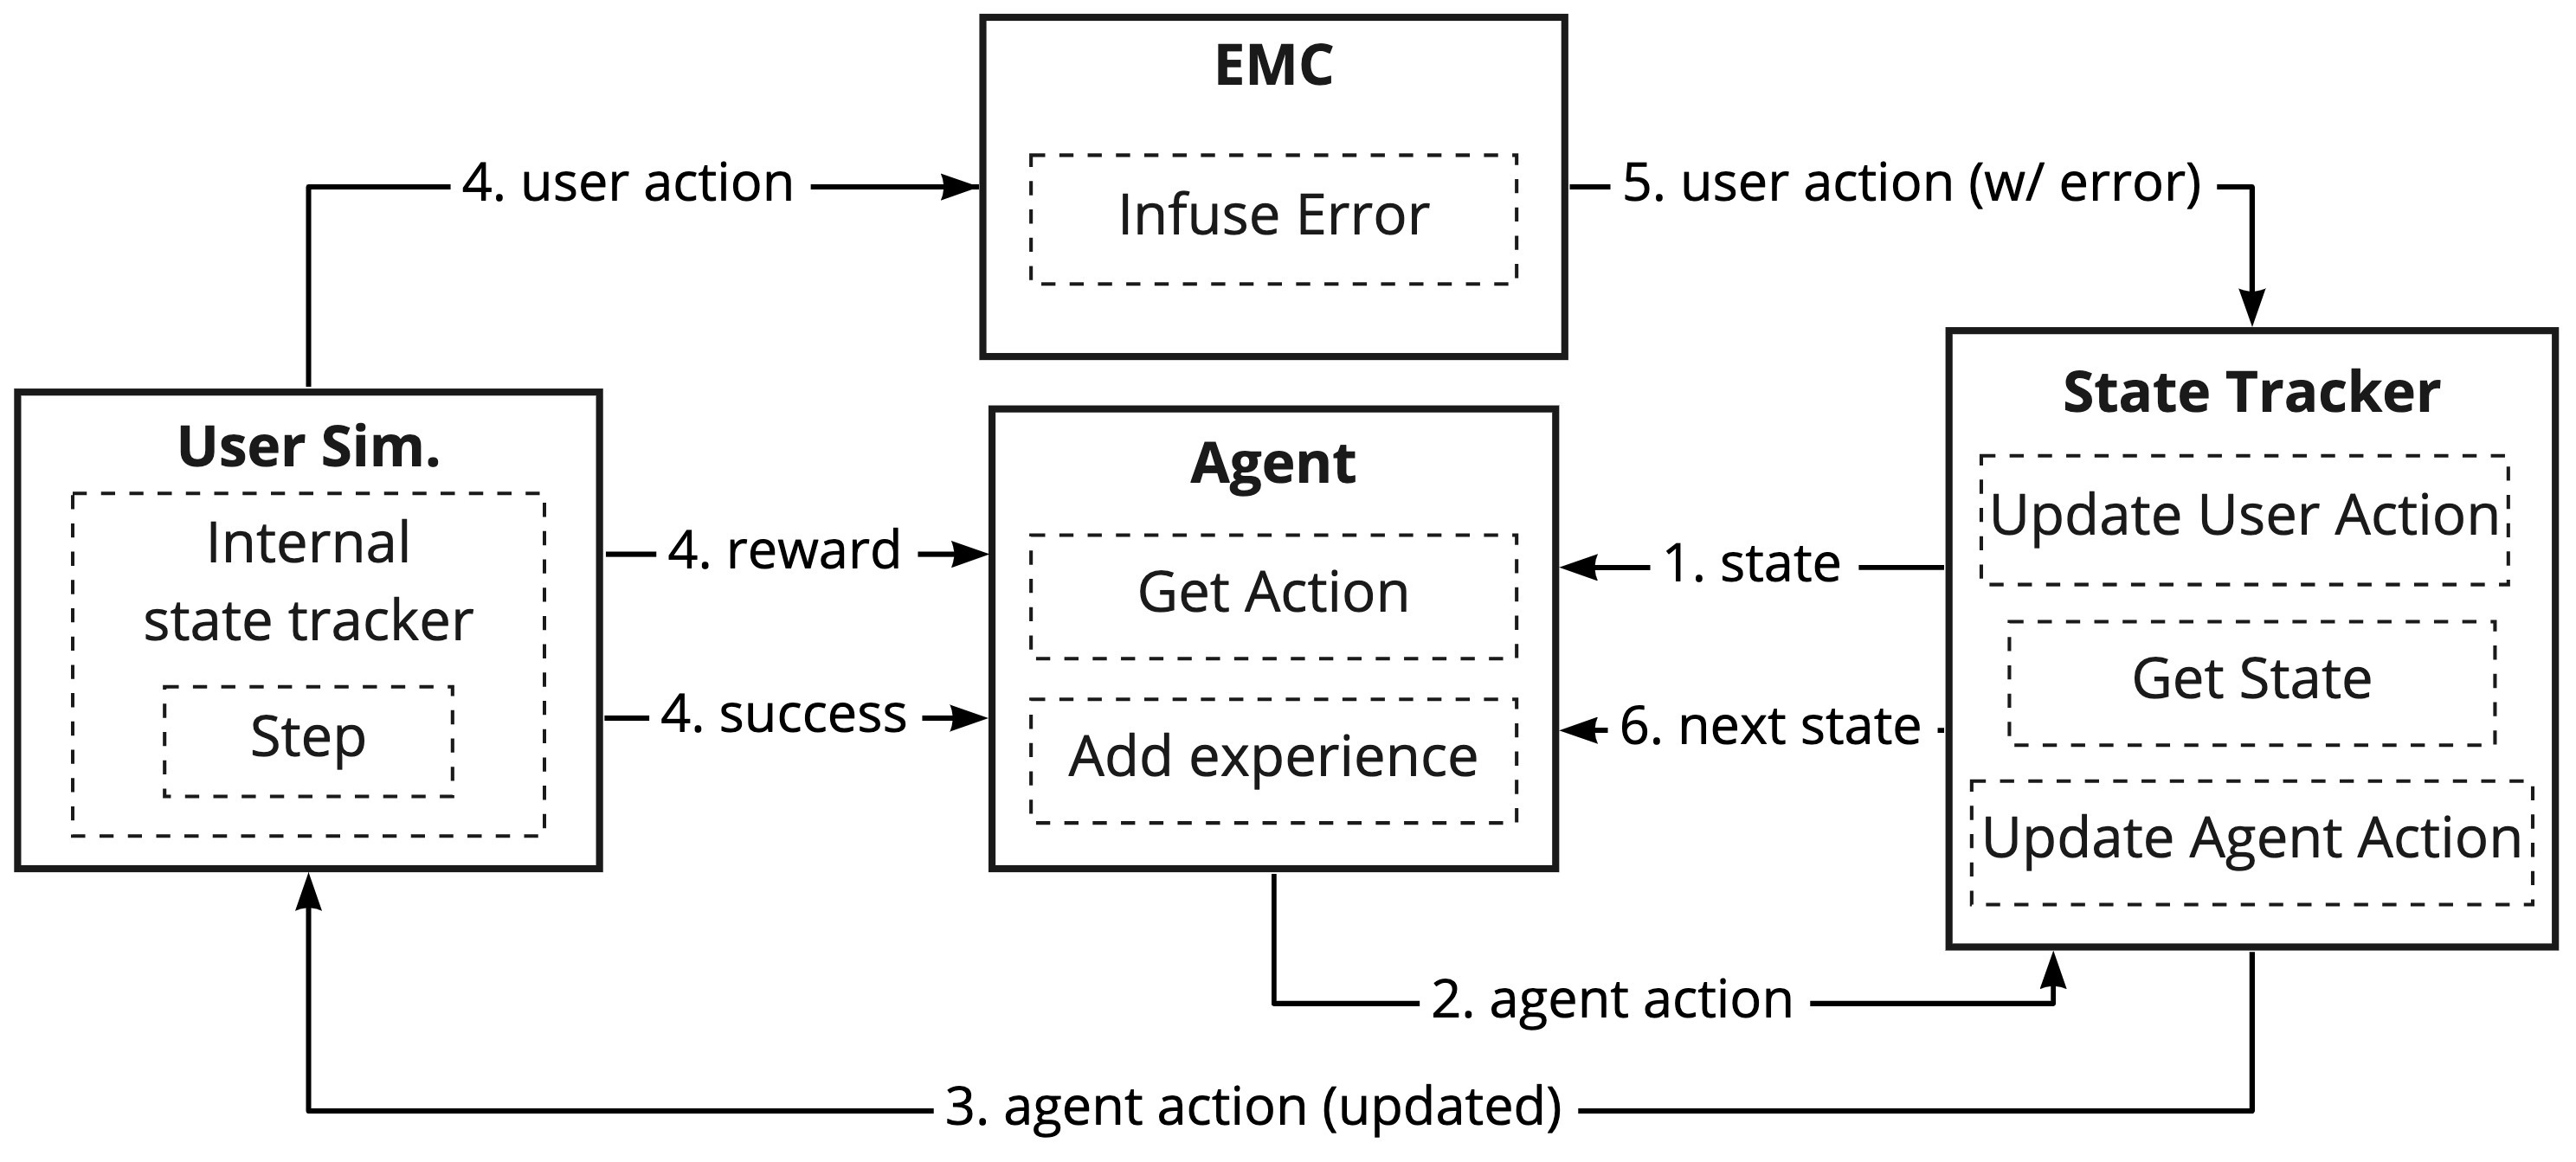
\includegraphics[scale=0.145]{thesis/chatbot/phuongphap/img/training.jpg}
    \caption{Vòng lặp huấn luyện - giai đoạn training}
    \label{fig:training}
\end{figure}

Mỗi một vòng thực hiện là một lượt đối thoại qua lại giữa người dùng
và tác nhân. Cụ thể:

\begin{itemize}
    \item \textbf{Bước 1:} Ta lấy ra \textit{state} - trạng thái
    hiện tại của hội thoại từ \textit{State Tracker} - bộ quản lý
    trạng thái hội thoại, trạng thái này có thể là trạng thái
    khởi tạo nếu như vừa bắt đầu hội thoại hoặc là trạng thái của
    toàn bộ cuộc hội thoại giữa người dùng và tác nhân. Trạng thái
    sau khi được lấy ra sẽ làm input (đầu vào) cho tác nhân ở
    bước tiếp theo.
    \item \textbf{Bước 2:} Tác nhân sau khi nhận được input từ
    bước trước sẽ sinh ra \textit{action} (hành động) và gửi ngược về
    lại bộ quản lý trạng thái hội thoại. Đồng thời ghi nhớ vào ký ức
    của nó. Hành động lúc này ở dạng thô, chưa kèm thông tin cụ thể.
    Nó sẽ được bộ quản lý trạng thái hội thoại cập nhật thông tin
    sau khi thực hiện truy vấn lên cơ sở dữ liệu cũng như cập nhật
    số lượt đã được thực hiện trong hội thoại. Đồng thời bộ quản lý
    trạng thái hội thoại cũng sẽ cập nhật lại trạng thái của hội thoại.
    \item \textbf{Bước 3:} Hành động sau khi được cập nhật đầy đủ
    thông tin sẽ được gửi cho bộ mô phỏng người dùng. Bộ mô phỏng
    người dùng sẽ dựa vào các luật đã được quy định trước để sinh ra
    hành động (có cấu trúc tương tự hành động của tác nhân ở
    bước trước), kèm theo \textit{reward} (điểm thưởng) và tín hiệu
    success (thành công) để giúp tác nhân có thể tự điều chỉnh
    hành vi để học. Ở đây, tác nhân cũng sẽ ghi lại toàn bộ vào
    ký ức của nó.
    \item \textbf{Bước 4:} Hành động của người dùng ở bước trước đó
    sẽ được đưa qua \textit{EMC} - bộ giả lập lỗi, trình bày cụ thể ở
    mục \ref{sec:emc}, mục đích là tạo ra các lỗi mà người dùng thật
    hay mắc phải, giúp tác nhân có hành vi chính xác và tự nhiên hơn
    khi chạy ở thực tế.
    \item \textbf{Bước 5:} Hành động ở bước trước sẽ tiếp tục được
    gửi đi đến bộ quản lý trạng thái hội thoại và được cập nhật
    thông tin cụ thể tương tự ở bước 2. Đồng thời bộ quản lý
    trạng thái hội thoại cũng cập nhật trạng thái của nó.
    \item \textbf{Bước 6:} Trạng thái tiếp theo được lấy từ bộ
    quản lý trạng thái hội thoại và quay lại giống bước 1.
\end{itemize}

Quá trình này sẽ được thực hiện liên tục cho đến khi tác nhân yêu cầu
kết thúc cuộc hội thoại sau khi nó nhận thấy đã hoàn thành yêu cầu
của người dùng hoặc khi số lượt hội thoại vượt quá mức ngưỡng quy định.

\subsubsection{Ví dụ}
Như trình bày ở trên, trong giai đoạn training, ta sẽ lấy ngẫu nhiên
một mục tiêu người dùng, được trình bày cụ thể ở mục
\ref{subsec:usergoal}, để làm mục tiêu cho bộ mô phỏng người dùng
trong suốt cuộc hội thoại. Xét một mẫu mục tiêu người dùng như sau:

\begin{itemize}
    \item Mục tiêu: yêu cầu thông tin sản phẩm
    \item Thông tin người dùng cung cấp trong hội thoại: tên sản phẩm
    \item Thông tin người dùng yêu cầu trong hội thoại: các màu
    khác nhau của sản phẩm
\end{itemize}

Giả sử, trạng thái chỉ chứa các ý định hành động hiện tại của
người dùng lần lượt là: hello, inform, request, reject, done.
Ta mã hóa về dạng one-hot vec-tơ để làm đầu vào cho mạng nơ-ron.
Quá trình huấn luyện trong giai đoạn training như sau:

\begin{itemize}
    \item Đầu tiên, bộ mô phỏng người dùng sẽ khởi tạo hành động
    đầu tiên trong hội thoại. Giả sử, nó tạo hành động như sau
    yêu cầu thông tin màu sắc và cung cấp tên sản phẩm
    (request(cost\_product), inform(name\_product)).
    Hành động này được đưa qua bộ giả lập lỗi. Giả sử, lỗi
    ngẫu nhiên được tạo là mất thông tin tên sản phẩm người dùng
    cung cấp. Hành động lúc này chỉ còn yêu cầu thông tin màu sắc
    (request(cost\_product)). Sau đó nó được gửi tới bộ quản lý
    trạng thái hội thoại. Bộ quản lý trạng thái hội thoại sẽ thêm
    thông tin số lượt thực hiện vào hành động của người dùng là 1
    để kiểm soát hội thoại kéo dài không quá số lượt cho phép (20).
    Đồng thời lấy trạng thái hiện tại của hội thoại gửi qua cho
    tác nhân là $[0\; 0\; 1\; 0\; 0]$. Quá trình được biểu diễn
    như hình \ref{fig:examtraining}.
\end{itemize}

\begin{figure}[ht!]
    \centering
    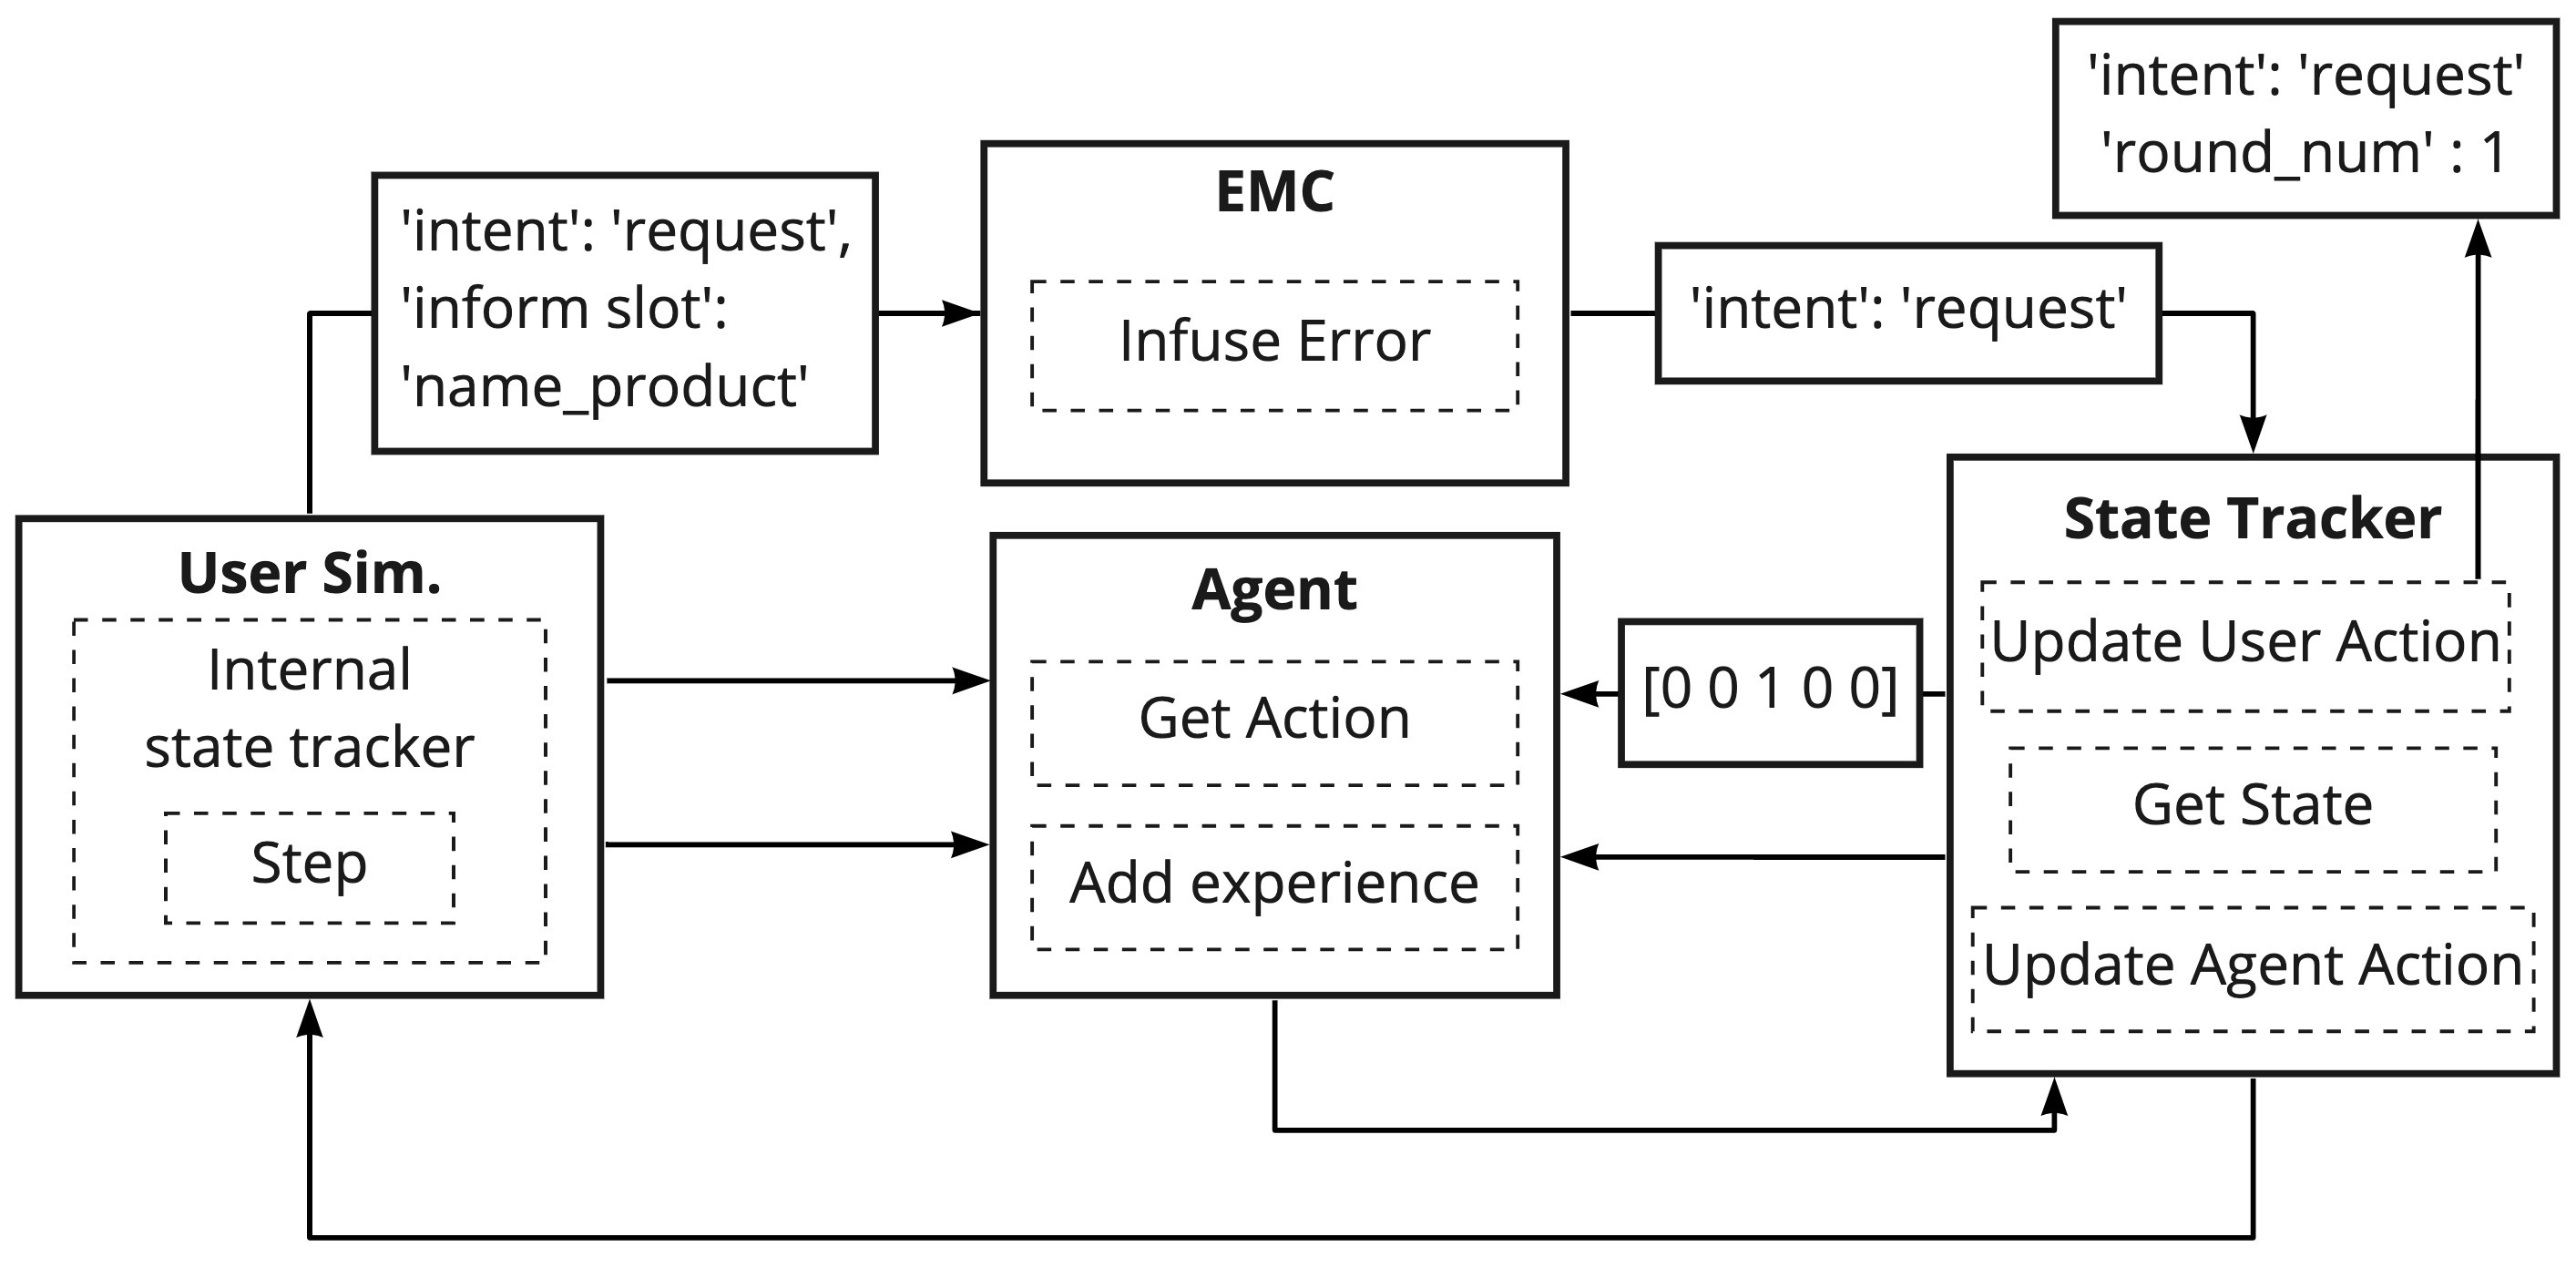
\includegraphics[scale=0.15]{thesis/chatbot/phuongphap/img/training_exam.jpg}
    \caption{Ví dụ quá trình huấn luyện bước 1 - giai đoạn training}
    \label{fig:examtraining}
\end{figure}

\begin{itemize}
    \item Tại đây, tác nhân sẽ đưa ra hành động có giá trị Q
    lớn nhất. Giả sử, ta có một mô hình với vộ trọng số như mục
    \ref{subsec:deepqlearning}, cho ra hành động kế tiếp là kết thúc
    hội thoại (done). Sau đó nó được gửi tới bộ quản lý trạng thái
    hội thoại. Tương tự, bộ quản lý trạng thái hội thoại sẽ thêm
    thông tin số lượt thực hiện vào hành động của tác nhân là 1 và
    gửi qua cho bộ mô phỏng người dùng. Quá trình được biểu diễn
    như hình \ref{fig:examtraining1}.
\end{itemize}

\begin{figure}[ht!]
    \centering
    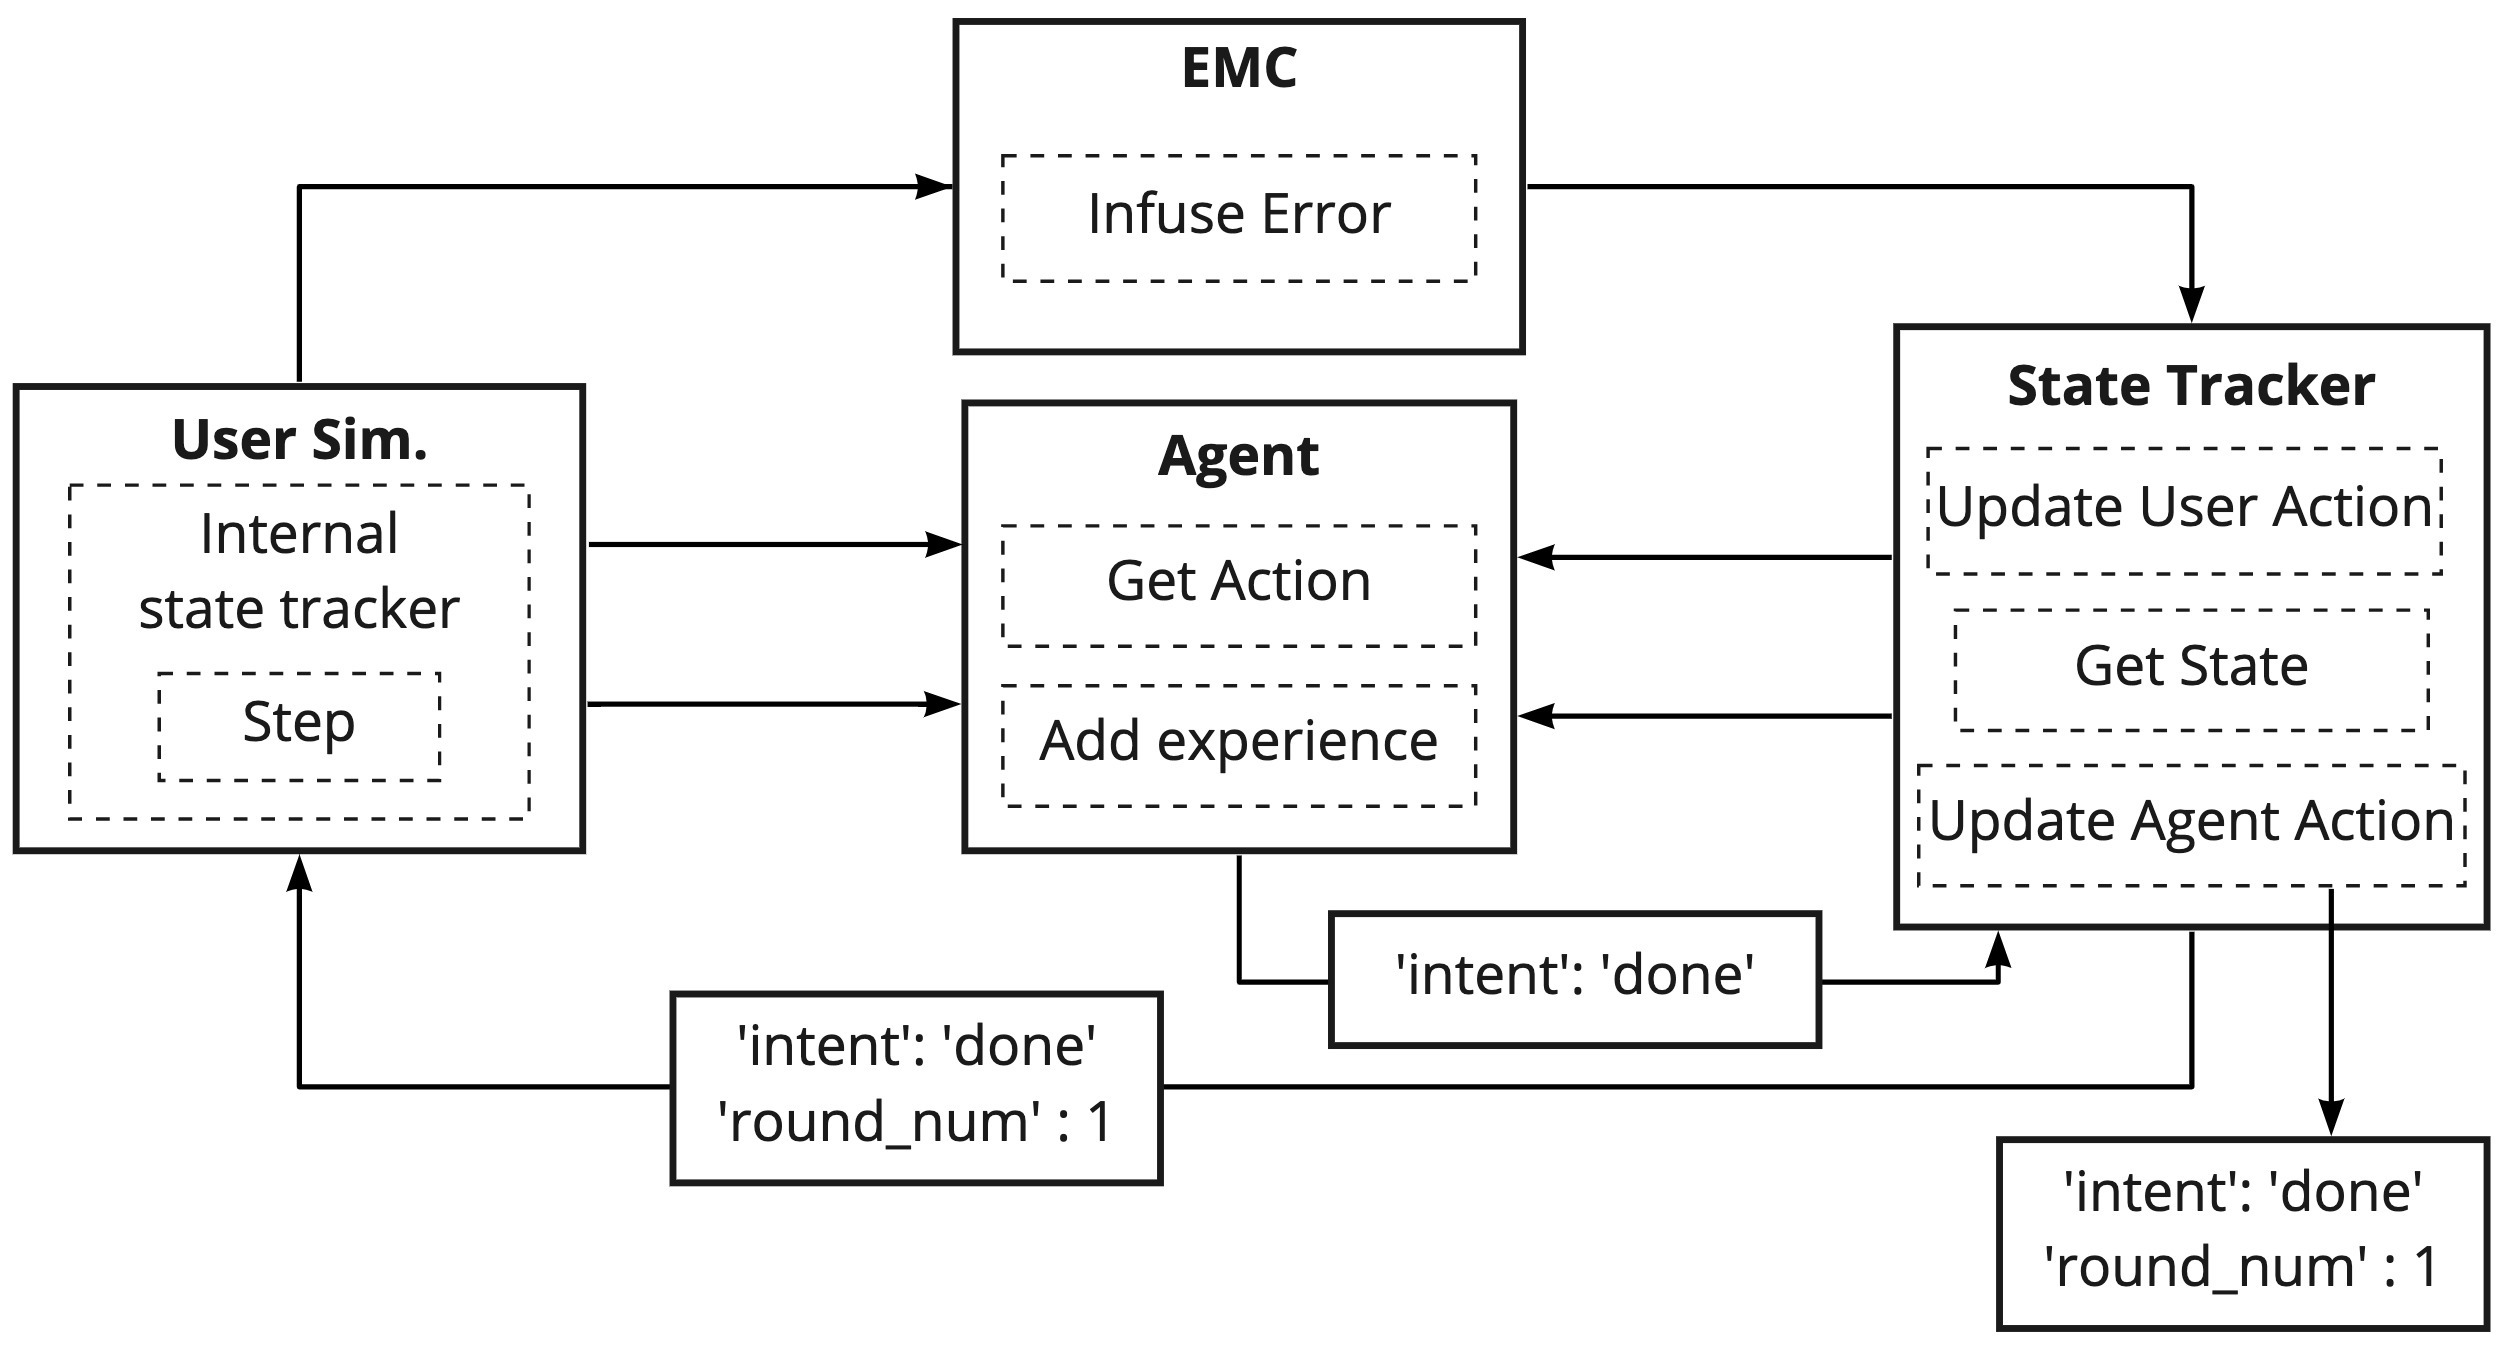
\includegraphics[scale=0.16]{thesis/chatbot/phuongphap/img/training_exam1.jpg}
    \caption{Ví dụ quá trình huấn luyện bước 2 - giai đoạn training}
    \label{fig:examtraining1}
\end{figure}

\begin{itemize}
    \item Hành động done là hành động kết thúc hội thoại của tác nhân
    mà nó chưa hoàn thành được mục tiêu cho người dùng. Vì vậy,
    với các luật quy định sẵn, bộ mô phỏng người dùng sẽ thực hiện
    hành động từ chối kết thúc hội thoại (reject), gửi tới bộ quản lý
    trạng thái hội thoại và gửi điểm thưởng là -10 cho tác nhân.
    Bộ quản lý trạng thái hội thoại sẽ thêm thông tin số lượt vào
    hành động của người dùng là 2. Cập nhật và lấy trạng thái hiện tại
    của hội thoại gửi qua cho tác nhân là $[0\; 0\; 0\; 1\; 0]$.
    Quá trình được biểu diễn như hình \ref{fig:examtraining2}.
\end{itemize}

\begin{figure}[ht!]
    \centering
    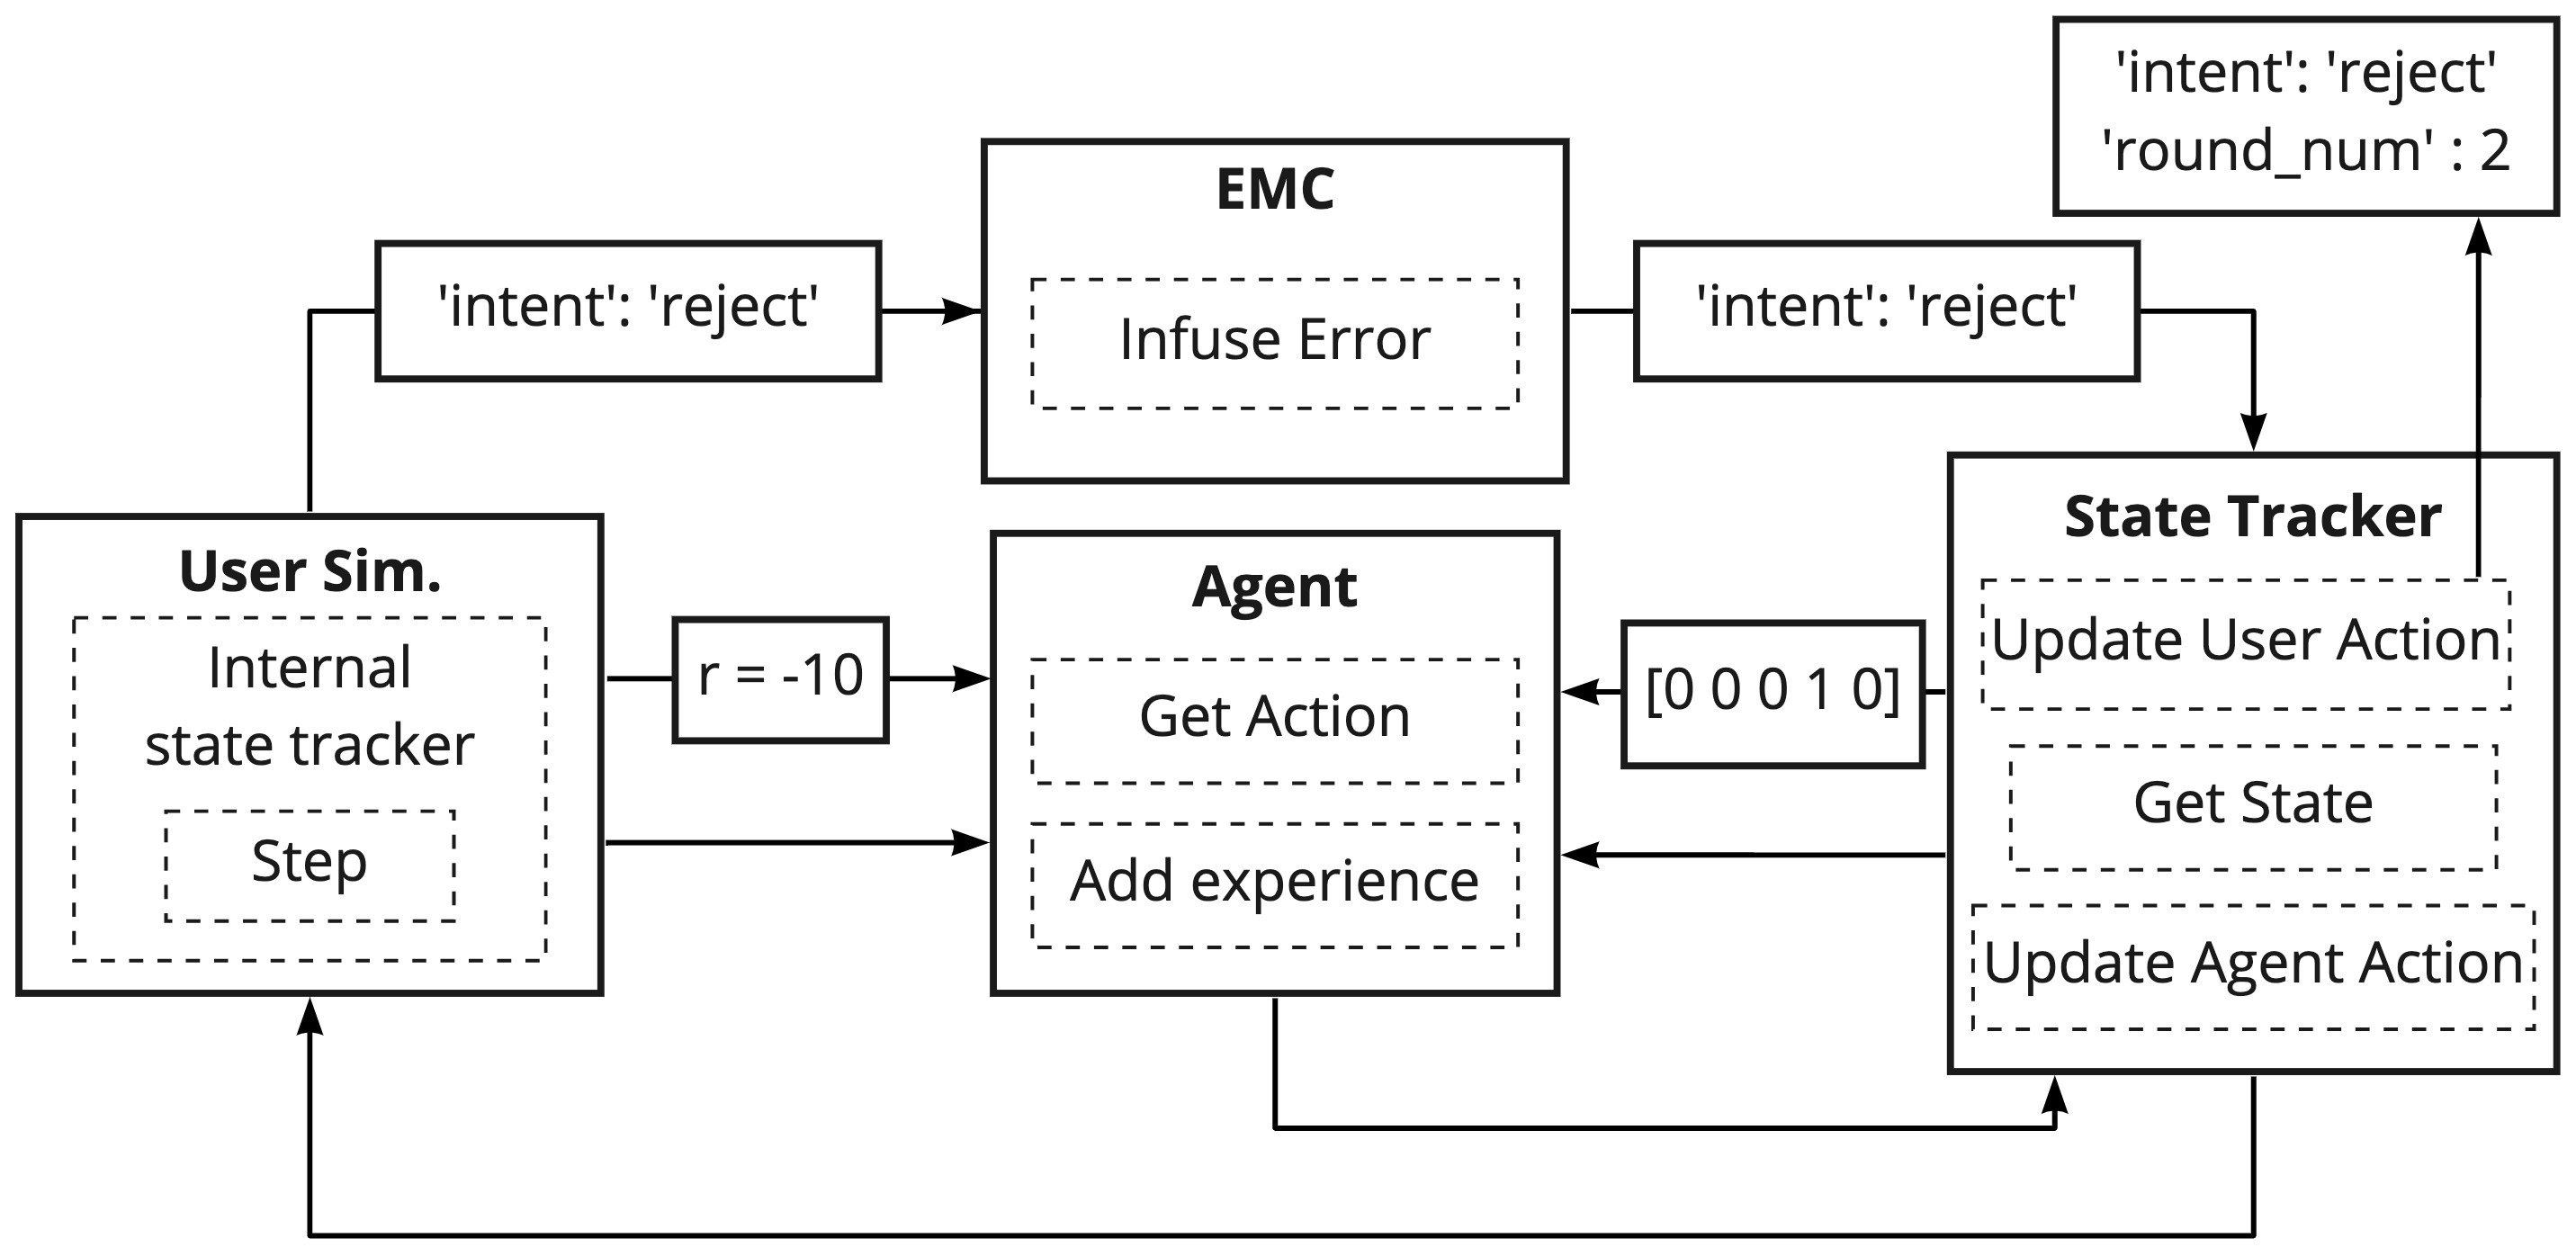
\includegraphics[scale=0.15]{thesis/chatbot/phuongphap/img/training_exam2.jpg}
    \caption{Ví dụ quá trình huấn luyện bước 3, 4 và 5 - giai đoạn training}
    \label{fig:examtraining2}
\end{figure}

Trạng thái hội thoại tại thời điểm này chính là trạng thái kế tiếp
của hành động trước đó (request(cost\_product),
inform(name\_product)) của người dùng.

Tại đây, chúng ta đã có đầy đủ thông tin:
\begin{itemize}
    \item State ($s$): trạng thái hiện tại khi người dùng yêu cầu
    thông tin và cung cấp tên sản phẩm (request(cost\_product),
    inform(name\_product)) là $[0\; 0\; 1\; 0\; 0]$.
    \item Next state ($s'$): trạng thái kế tiếp của người dùng
    sau khi tác nhân phản hồi yêu cầu kết thúc hội thoại (done)
    là $[0\; 0\; 0\; 1\; 0]$.
    \item Action ($a$): hành động tác nhân phản hồi tại
    trạng thái $s$ là done.
    \item Reward ($r_0$): phần thưởng cho hành động $a$ là -10.
\end{itemize}

Toàn bộ thông tin này được lưu vào bộ nhớ. Khác với giai đoạn warm-up.
Ta thực hiện việc huấn luyện như mô tả ở mục \ref{subsec:deepqlearning}
sau một số các hội thoại kết thúc được xác định trước.

\section{Vấn đề cần giải quyết}
Đề tài này có những vấn đề sau cần giải quyết:

\begin{itemize}
    \item Thu thập và chọn lọc các dữ liệu ban đầu vào cơ sở dữ liệu
    từ danh sách các thông tin sản phẩm của cửa hàng. Các dữ liệu về
    kích cỡ sản phẩm phù hợp với cơ thể người từ bảng kích cỡ của cửa hàng.
    \item Xác định các ý định của người dùng.
    \item Xây dựng được một bộ quản lý hội thoại cho Chatbot sao cho
    quá trình hội thoại được diễn ra tự nhiên và vẫn đáp ứng được
    nhu cầu tư vấn của người dùng.
    \item Xây dựng được một bộ phản hồi cho Chatbot sao cho các câu
    phản hồi tự nhiên và sát với con người nhất có thể, không tạo
    cảm giác quá rập khuôn hay cứng nhắc.
    \item Xây dựng được một trang web tích hợp các thành phần trong
    hệ thống thành Chatbot, có giao diện đơn giản, dễ sử dụng.
    \item Triển khai hệ thống và thu thập ý kiến đánh giá từ
    người dùng Chatbot.
\end{itemize}

\section{Khó khăn}
Trong quá trình giải quyết các vấn đề gặp phải các khó khăn sau:

\begin{itemize}
    \item Dữ liệu về bảng kích cỡ sản phẩm với số đo cơ thể người còn
    hạn chế, ảnh hưởng đến truy vấn tìm kiếm các thông tin phù hợp.
    \item Dữ liệu nhập bởi người dùng có thể có nhiều dạng khác nhau,
    việc chuẩn hóa thông tin đòi hỏi nhiều thời gian để nghiên cứu
    và thực hiện.
    \item Việc huấn luyện cho tác nhân gặp nhiều khó khăn ở bước đầu.
    Tác nhân phản hồi không hợp lý, cần nhiều thời gian để thử nghiệm
    trên các tập dữ liệu và điều chỉnh luật huấn luyện phù hợp.
\end{itemize}

\section{Giải pháp}
Để giải quyết các khó khăn đã nêu trên, đề xuất ra các giải pháp sau:

\begin{itemize}
    \item Nhờ sự giúp đỡ từ các cộng tác viên, và thông tin trực tiếp
    từ cửa hàng, cập nhật dữ liệu được đầy đủ và chính xác.
    \item Xây dựng bộ chuẩn hóa dữ liệu nhập vào theo giai đoạn,
    cải tiến từng phần dựa trên trải nghiệm thực tế.
    \item Phân tích, tìm hiểu rõ thuật toán và nguyên lý hoạt động
    của mô hình huấn luyện học tăng cường để tiến hành điều chỉnh các
    thông số, tập dữ liệu sao cho thích hợp và mang lại
    kết quả chính xác, đúng yêu cầu đặt ra.
\end{itemize}
